% =====================================================================
%  Báo cáo đồ án cuối kỳ — Phân tích dữ liệu thông minh
%  Tác động của việc giảm thuế GTGT 10% -> 8% lên giá bán lẻ
%
%  Biên dịch: pdflatex main.tex  (chạy 2 lần để mục lục đúng)
%  Hình nằm trong thư mục hinh/, chép từ ket-qua/hinh/ của repo.
%
%  LƯU Ý VỀ SỐ LIỆU
%  Toàn bộ con số trong file này được GÕ TAY từ các file kết quả trong
%  ket-qua/. Khác với web và slide (đọc thẳng từ pipeline nên không thể
%  lệch), báo cáo này KHÔNG tự cập nhật khi chạy lại pipeline. Nếu chạy
%  lại code, phải đối chiếu tay các bảng dưới đây với ket-qua/*.csv.
%  Mỗi bảng đều ghi rõ nguồn ở phần chú thích để đối chiếu cho nhanh.
% =====================================================================
\documentclass[11pt]{article}

\usepackage[utf8]{inputenc}
\usepackage[T5]{fontenc}
\usepackage[vietnamese]{babel}
\usepackage[a4paper,margin=2.5cm]{geometry}
\usepackage{amsmath}
\usepackage{amssymb}
\usepackage{graphicx}
\usepackage{enumitem}
\usepackage{booktabs}
\usepackage{multirow}
\usepackage{array}
\usepackage{caption}
\usepackage{hyperref}

\hypersetup{
  unicode=true,
  hidelinks,
  pdfauthor={Nhom 5 - PTDLTM},
  pdftitle={Tac dong cua viec giam thue GTGT len gia ban le}
}
\setlist{leftmargin=*}
\emergencystretch=3em

% Lệnh viết tắt cho đơn vị dùng suốt báo cáo.
\newcommand{\dvi}{điểm log $\times$100}

\begin{document}

%================= TRANG BÌA =================
\begin{titlepage}
  \centering
  {\large\scshape Trường Đại học Khoa học Tự nhiên, ĐHQG-HCM\par}
  {\large\scshape Khoa Công nghệ Thông tin\par}
  \vspace{0.4cm}
  \rule{\linewidth}{0.4pt}

  \vfill

  {\large Báo cáo đồ án cuối kỳ\par}
  \vspace{0.3cm}
  {\large Phân tích Dữ liệu Thông minh (PTDLTM)\par}

  \vspace{1.6cm}

  {\Huge\bfseries Tác động của việc giảm thuế GTGT\\[0.3em] lên giá bán lẻ\par}

  \vspace{1.0cm}
  \rule{0.6\linewidth}{0.4pt}
  \vspace{0.8cm}

  {\large\itshape Đánh giá thực nghiệm chính sách giảm thuế GTGT\\
   từ 10\% xuống 8\% theo Nghị quyết 204/2025/QH15\par}
  \vspace{0.3cm}
  {\normalsize Dữ liệu hóa đơn điện tử của một cửa hàng tiện lợi tại TP.HCM,\\
   12/2024 -- 08/2025\par}

  \vfill

  {\large\bfseries Nhóm thực hiện\par}
  \vspace{0.6cm}
  {\renewcommand{\arraystretch}{1.3}%
  \begin{tabular}{ll}
    Nguyễn Đình Lộc & \texttt{25C11050} \\
    Dương Tiến Vinh & \texttt{24C11034} \\
    Phạm Thị Chiều  & \texttt{24C12003} \\
    Lê Hoàng Nhân   & \texttt{24C11044} \\
  \end{tabular}\par}

  \vspace{0.8cm}
  {\large Giảng viên hướng dẫn: TS. Bùi Tiến Lên\par}

  \vfill

  {\large Thành phố Hồ Chí Minh, 2025\par}
\end{titlepage}

%================= TÓM TẮT =================
\begin{abstract}
\noindent
Nghị quyết 204/2025/QH15 giảm thuế giá trị gia tăng từ 10\% xuống 8\% kể từ 01/07/2025. Báo cáo
này trả lời câu hỏi: phần thuế được giảm có thật sự đi vào giá bán lẻ mà người tiêu dùng chi trả
hay không. Dữ liệu là toàn bộ hóa đơn điện tử của một cửa hàng tiện lợi tại TP.HCM giai đoạn
12/2024--08/2025, gồm 233.996 dòng hàng. Vì luật cho giảm thuế nhóm hàng tiêu dùng thông thường
nhưng loại trừ hàng chịu thuế tiêu thụ đặc biệt (rượu, bia, thuốc lá), dữ liệu chứa sẵn một nhóm
can thiệp và một nhóm đối chứng trong cùng cửa hàng, cùng khoảng thời gian --- một
\emph{thí nghiệm tự nhiên}. Nhóm dùng hai mô hình phân tích nhân quả khác nhau: hồi quy có điều
chỉnh hiệp biến và phân tầng theo phân vị giá nền, cộng thêm hai biến thể để so sánh. Bốn ước
lượng cho chênh lệch từ $-0{,}257$ đến $-0{,}664$ \dvi{}, tương ứng 14\%--36\% mức chuyển hoàn
toàn, nhưng cả bốn khoảng tin cậy 95\% đều phủ qua 0. Ba cổng chẩn đoán đặt trước cho thấy giả
định xu hướng song song không được xác nhận, nên các ước lượng này được trình bày là
\emph{so sánh có điều chỉnh}. Song song đó, một phép đối chiếu cơ học không cần nhóm đối chứng
cho thấy: trong 135 mặt hàng lẽ ra phải đổi giá nếu giảm đúng theo phần thuế, chỉ \textbf{1} mặt
hàng rơi đúng mức đó và \textbf{110} mặt hàng giữ nguyên giá cũ. Kết luận trung tâm của đồ án là
cửa hàng đã \emph{không} chuyển hết phần giảm thuế vào giá bán lẻ; các giới hạn về thiết kế ảnh
hưởng tới \emph{độ lớn} ước lượng được chứ không lật ngược phát hiện này.
\end{abstract}

%================= MỤC LỤC =================
\newpage
\tableofcontents
\newpage

% =====================================================================
\section{Giới thiệu}
% =====================================================================

\subsection{Bối cảnh và động cơ}

Nhà nước giảm thuế giá trị gia tăng (GTGT) nhằm hỗ trợ người tiêu dùng. Thuế này nằm trong số
tiền người mua trả khi thanh toán, nên kỳ vọng tự nhiên là giá thanh toán cũng giảm theo.

Tuy vậy, thuế suất giảm \emph{không} kéo theo việc giá bán tự động giảm đúng bằng phần thuế được
giảm. Nhà nước quyết định thuế suất, nhưng cửa hàng mới là bên quyết định giá niêm yết và thời
điểm cập nhật giá. Hai quyết định này độc lập với nhau. Vì vậy, câu hỏi thay đổi chính sách có
thật sự xuất hiện trong số tiền khách hàng trả hay không là một câu hỏi thực nghiệm, không phải
một suy luận hiển nhiên.

Đề tài phù hợp với môn học vì nó cho phép đi từ dữ liệu giao dịch thật đến một câu hỏi nhân quả
cụ thể. Hóa đơn điện tử ghi rõ từng mặt hàng đã bán, thuế suất được áp và số tiền sau thuế --- đủ
để theo dõi cùng một mã hàng trước và sau ngày chính sách có hiệu lực.

\subsection{Câu hỏi nghiên cứu}

\begin{quote}
\textbf{Việc giảm thuế GTGT từ 10\% xuống 8\% ngày 01/07/2025 có làm giảm giá bán lẻ mà người tiêu
dùng thực trả tại cửa hàng được khảo sát không?}
\end{quote}

Cần phân biệt ba đại lượng thường bị gộp làm một:

\begin{table}[htbp]
  \centering
  \caption{Ba đại lượng cần tách bạch.}
  \label{tab:ba-dai-luong}
  \begin{tabular}{ll}
    \toprule
    Đại lượng & Ý nghĩa \\
    \midrule
    Giá chưa thuế         & Doanh thu về tay cửa hàng \\
    Quyết định định giá   & Cửa hàng chọn niêm yết bao nhiêu \\
    Giá gồm thuế          & Số tiền người tiêu dùng thực trả \\
    \bottomrule
  \end{tabular}
\end{table}

Chính sách tác động trực tiếp lên \emph{thuế suất}. Việc nó có tới được \emph{giá gồm thuế} hay
không phụ thuộc quyết định định giá của cửa hàng. Đó chính là nội dung của khái niệm
\textbf{pass-through} --- tỉ lệ phần thuế được giảm thực sự đi vào giá bán.

Đồ án quan tâm trước hết đến giá gồm thuế, vì đây là số tiền người mua nhìn thấy trên hóa đơn.
Giá chưa thuế được xem xét bổ sung để hiểu cách tổng số tiền được chia lại giữa thuế và doanh thu.

\subsection{Phạm vi}

Dữ liệu chỉ đến từ \textbf{một cửa hàng tiện lợi tại TP.HCM}. Kết quả vì vậy mô tả cách cửa hàng
này định giá trong giai đoạn được quan sát.

\begin{quote}
\textbf{Cảnh báo phạm vi.} Không được ngoại suy kết quả ra cửa hàng khác hoặc ra toàn ngành. Đồ án
có một cửa hàng, một ngày chính sách và một người ra quyết định giá.
\end{quote}

Phạm vi hẹp này đổi lại cho phép theo dõi \emph{cùng một mã hàng} trước và sau chính sách --- điều
kiện then chốt để loại bỏ thay đổi cơ cấu mặt hàng khỏi phép so sánh.

\subsection{Đóng góp của đồ án}

\begin{itemize}
  \item Xây dựng một \textbf{thiết kế thí nghiệm tự nhiên có không tuân thủ} từ dữ liệu hóa đơn
  thực địa, tách bạch \emph{đủ điều kiện theo luật} khỏi \emph{thuế suất cửa hàng thực áp}.
  \item Áp dụng \textbf{hai mô hình phân tích nhân quả khác nhau} --- hồi quy có điều chỉnh và
  phân tầng theo phân vị giá --- cùng hai biến thể để so sánh chéo, và chỉ ra chính xác điều gì
  khiến bốn con số khác nhau.
  \item Đặt \textbf{ba cổng chẩn đoán trước khi chạy} và báo cáo trung thực việc hai trong ba cổng
  không đạt, thay vì trình bày kết quả như một ước lượng nhân quả sạch.
  \item Bổ sung một \textbf{phép đối chiếu cơ học} không cần nhóm đối chứng và không cần giả định
  nhận dạng nào, cho phép kết luận về mức độ thực thi chính sách ở cấp cửa hàng.
\end{itemize}

% =====================================================================
\section{Cơ sở pháp lý}
% =====================================================================

\subsection{Chính sách được nghiên cứu}

Nghị quyết 204/2025/QH15~\cite{nq204} tiếp tục giảm thuế GTGT từ \textbf{10\% xuống 8\%}, hiệu lực
từ \textbf{01/07/2025}. Trước đó, chính sách giảm thuế được thực hiện theo Nghị quyết
174/2024/QH15~\cite{nq174}.

Hai nghị quyết không chỉ xác định thời điểm áp dụng. Chúng còn xác định mặt hàng nào được giảm và
mặt hàng nào tiếp tục chịu thuế suất 10\%. Đây chính là phần cho phép chia dữ liệu thành hai nhóm
so sánh.

\subsection{Diện được giảm và diện loại trừ}

Trong phạm vi dữ liệu của cửa hàng, đồ án tập trung vào hai nhóm:

\begin{itemize}
  \item \textbf{Nhóm đủ điều kiện} được giảm thuế theo Nghị quyết 204/2025/QH15. Nghị quyết này bỏ
  ``sản phẩm hóa chất'' khỏi danh mục loại trừ, nên nhóm hóa chất tẩy rửa và mỹ phẩm chuyển từ 10\%
  xuống 8\%.
  \item \textbf{Nhóm bị loại trừ} --- hàng chịu thuế tiêu thụ đặc biệt, gồm rượu, bia và thuốc lá.
  Nhóm này bị loại trừ ở \emph{cả hai} nghị quyết nên giữ thuế suất 10\% suốt kỳ.
\end{itemize}

Việc phân nhóm dựa trên \emph{quy định pháp lý và loại sản phẩm}, không dựa trên việc giá của mặt
hàng đã tăng hay giảm. Điều này quan trọng: nếu chia nhóm theo kết quả giá thì phép so sánh sẽ
mang tính vòng tròn.

\subsection{Vì sao đây là một thí nghiệm tự nhiên}

Quyết định mặt hàng nào được giảm thuế do \emph{Quốc hội} ban hành, không do cửa hàng lựa chọn.
Vì vậy, trong cùng một cửa hàng và cùng một khoảng thời gian, dữ liệu có sẵn một nhóm được chính
sách cho giảm thuế và một nhóm không được giảm --- một nguồn biến thiên ngoại sinh với hành vi
định giá.

Tuy nhiên, cửa hàng có thể cập nhật thuế và giá không hoàn toàn khớp quy định. Vì thế báo cáo tách
\emph{đủ điều kiện theo luật} khỏi \emph{thuế suất cửa hàng thực áp}; chi tiết ở
mục~\ref{sec:khong-tuan-thu}.

\subsection{Mốc chuyển hoàn toàn}
\label{sec:moc-chuyen}

Nếu giá chưa thuế của một mặt hàng không đổi, giá khách trả chỉ thay đổi do thuế suất:
\begin{equation}
  \frac{\text{giá sau}}{\text{giá trước}} = \frac{1{,}08}{1{,}10}
  \qquad\Longrightarrow\qquad
  \frac{1{,}08}{1{,}10} - 1 = -1{,}82\%.
  \label{eq:moc-phan-tram}
\end{equation}

Mức $-1{,}82\%$ là \textbf{mốc chuyển hoàn toàn} được dùng suốt báo cáo: nếu toàn bộ phần giảm
thuế đi vào giá bán và giá chưa thuế giữ nguyên, người mua sẽ trả ít hơn đúng mức này.

Vì các mô hình ở mục~\ref{sec:ket-qua} làm việc trên thang log, cùng một mốc được viết lại thành
\begin{equation}
  \tau_{\text{full}} = 100 \times \log\!\left(\frac{1{,}08}{1{,}10}\right) = -1{,}835 \ \text{\dvi}.
  \label{eq:moc-log}
\end{equation}
Hai cách viết khác thang đo nhưng mô tả cùng một thay đổi thuế.

% =====================================================================
\section{Dữ liệu}
% =====================================================================

\subsection{Nguồn và quy mô}

Dữ liệu là hóa đơn điện tử của một cửa hàng tiện lợi tại TP.HCM, trích từ phần mềm kế toán và lưu
trong file \texttt{60.xlsx}. File gồm một bảng thông tin hóa đơn và một bảng chi tiết từng dòng
hàng, nối với nhau bằng mã hóa đơn. Mỗi dòng chi tiết cho biết mặt hàng, số lượng, thành tiền,
thuế suất và mã vạch. Mã vạch được dùng để nhận diện SKU --- một mã hàng cụ thể.

Dữ liệu trải từ 12/2024 đến 08/2025. Quy mô cần đọc theo \textbf{bốn thang bậc} khác nhau:

\begin{table}[htbp]
  \centering
  \caption{Bốn thang bậc quan sát. Nguồn: \texttt{bang-luong-mau.csv} và
  \texttt{manifest-tai-lap.json}.}
  \label{tab:quy-mo}
  \begin{tabular}{lrl}
    \toprule
    Thang bậc & Quy mô & Nghĩa \\
    \midrule
    Dòng hàng thô              & 233.996 & Một mặt hàng trên một hóa đơn \\
    Dòng hàng sau lọc          & 82.109  & Các dòng đi vào danh mục phân tích \\
    SKU trong danh mục phân tích & 2.218 & Mã hàng còn lại sau khi dựng danh mục \\
    SKU trong mẫu so sánh chính  & 287   & Mã hàng thuộc hai nhóm $Z$ được so sánh \\
    \bottomrule
  \end{tabular}
\end{table}

Dữ liệu có hơn 2.000 quan sát ở cả cấp dòng hàng lẫn cấp danh mục SKU. Con số 287 là tập con cuối
dùng cho phép so sánh chính, không phải toàn bộ dữ liệu đầu vào.

\textbf{Đơn vị phân tích nhân quả là SKU sai phân trước--sau}, không phải dòng hóa đơn. Câu hỏi
nghiên cứu nói về quyết định định giá \emph{theo mặt hàng}, nên mỗi SKU được đếm đúng một lần; các
dòng hóa đơn chỉ dùng để dựng giá của SKU trong từng kỳ.

\subsection{Độ phủ dữ liệu không đều}

\begin{table}[htbp]
  \centering
  \caption{Độ phủ dữ liệu theo tháng. Nguồn: \texttt{eda-do-phu-theo-thang.csv}.}
  \label{tab:do-phu}
  \begin{tabular}{lrrrrr}
    \toprule
    Tháng & Ngày có dữ liệu & Hóa đơn & Dòng hàng & Có mã vạch & SKU \\
    \midrule
    12/2024 & 13 & 31     & 21.564 & 0\%   & --- \\
    01/2025 & 12 & 34     & 22.842 & 0\%   & --- \\
    02/2025 & 18 & 6.554  & 25.512 & 0\%   & --- \\
    03/2025 & 11 & 4.498  & 11.572 & 0\%   & --- \\
    04/2025 & 10 & 4.954  & 16.212 & 100\% & 1.994 \\
    05/2025 & 28 & 12.481 & 31.890 & 100\% & 2.357 \\
    06/2025 & 21 & 8.857  & 23.506 & 100\% & 2.405 \\
    07/2025 & 31 & 10.855 & 28.934 & 100\% & 2.452 \\
    08/2025 & 17 & 5.963  & 16.329 & 100\% & 2.096 \\
    \bottomrule
  \end{tabular}
\end{table}

Ba điểm phải nói rõ ngay:

\begin{itemize}
  \item Dữ liệu có một lỗ hổng \textbf{39 ngày}, từ 13/03 đến 20/04/2025.
  \item Tháng 06 thiếu thêm \textbf{9 ngày liên tiếp}, từ 02/06 đến 10/06. Ngày 12/06 có 2.781 hóa
  đơn, gấp khoảng 8 lần ngày thường --- nhiều khả năng là giao dịch được nhập bù sau khi cửa hàng
  mở lại.
  \item Mã vạch chỉ bắt đầu được điền từ \textbf{21/04/2025}. Các tháng trước đó không thể dùng để
  theo dõi cùng một SKU.
\end{itemize}

Dữ liệu cho thấy hai mốc quan sát được: khoảng trống 02--10/06, và địa chỉ trên hóa đơn đổi hẳn từ
24/06. Dữ liệu \emph{không} xác định được ngày cửa hàng dời địa điểm vật lý. Phân tích chính dùng
tháng 05--06 làm tiền kỳ và 07--08 làm hậu kỳ; cửa sổ từ 11/06 gồm cả hai địa chỉ được báo cáo
riêng ở phần độ nhạy.

\begin{figure}[htbp]
  \centering
  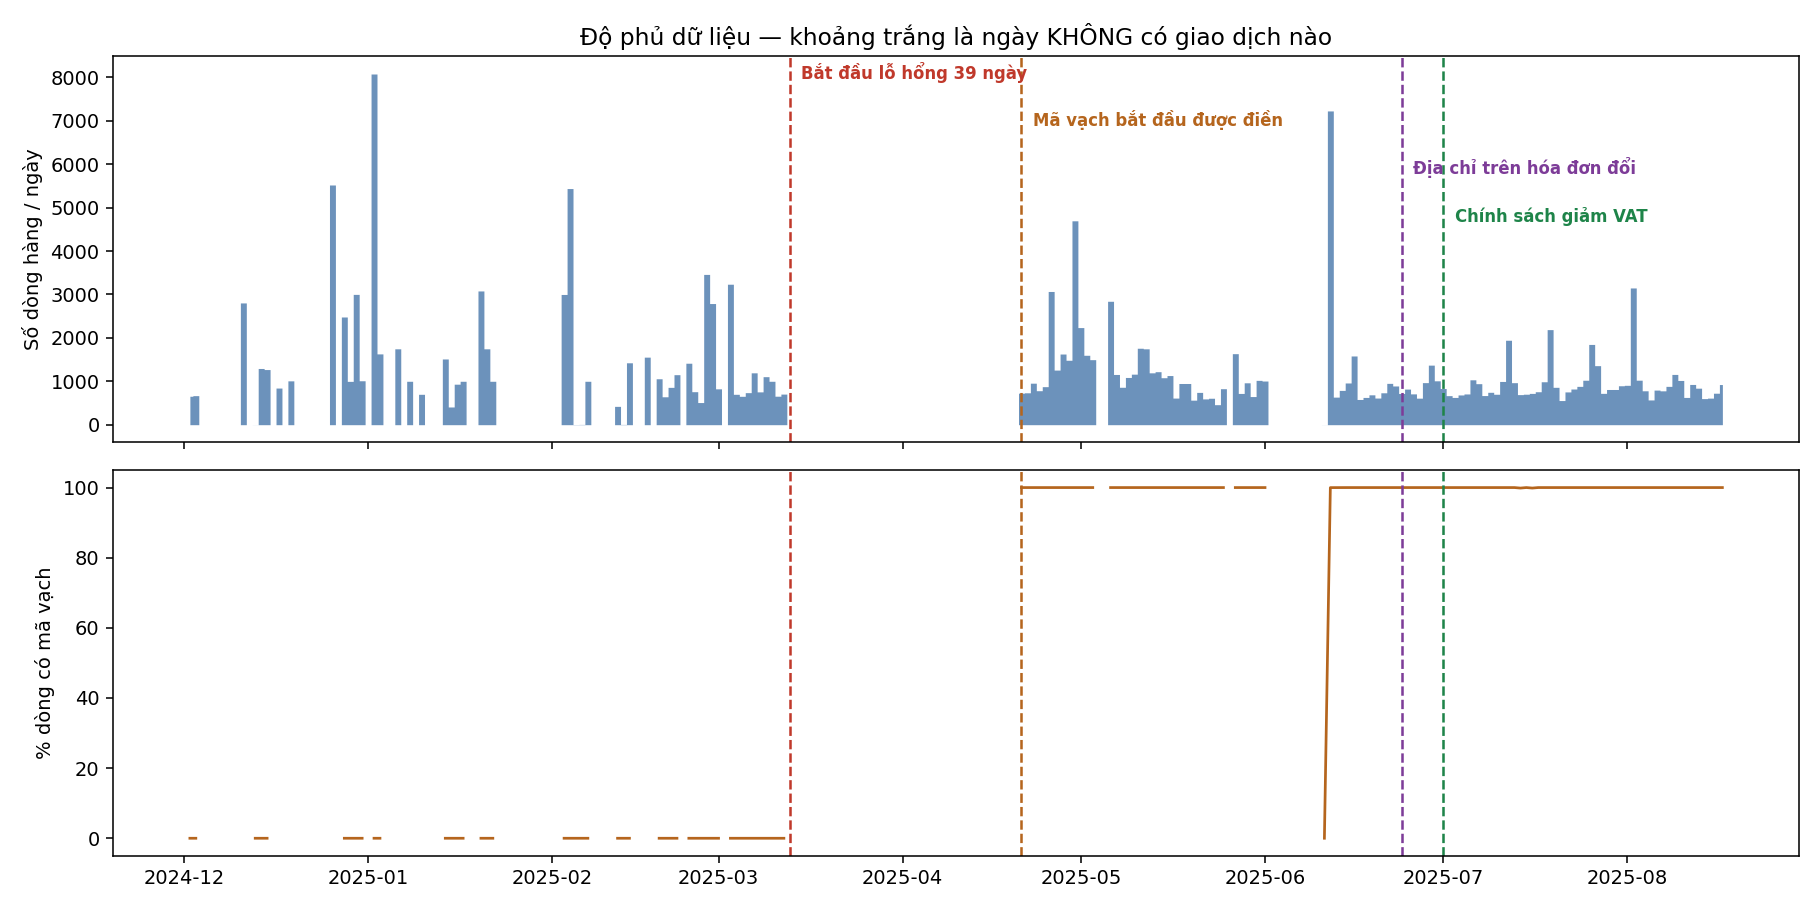
\includegraphics[width=\linewidth]{hinh/eda-do-phu-du-lieu.png}
  \caption{Độ phủ dữ liệu theo thời gian. Hình cho thấy các đoạn thiếu dữ liệu, thời điểm mã vạch
  bắt đầu xuất hiện, mốc địa chỉ trên hóa đơn đổi và ngày chính sách có hiệu lực.}
  \label{fig:do-phu}
\end{figure}

\subsection{Từ dữ liệu thô đến mẫu phân tích}

Việc làm sạch đi theo một luồng cố định, mỗi bước ghi rõ quy tắc và số dòng bị loại.

\begin{table}[htbp]
  \centering
  \caption{Luồng lọc mẫu. Nguồn: \texttt{bang-luong-mau.csv}.}
  \label{tab:luong-mau}
  \begin{tabular}{rlrrr}
    \toprule
    Bước & Quy tắc & Dòng vào & Dòng ra & Bị loại \\
    \midrule
    0  & Dữ liệu thô của bảng chi tiết        & 233.996 & 233.996 & 0 \\
    1  & Nối với bảng hóa đơn theo mã hóa đơn & 233.996 & 233.996 & 0 \\
    2  & Chỉ giữ hóa đơn bán ra               & 233.996 & 198.361 & 35.635 \\
    3  & Bỏ bản ghi có cờ xóa                 & 198.361 & 188.416 & 9.945 \\
    4  & Giữ dữ liệu từ 01/04/2025            & 188.416 & 106.926 & 81.490 \\
    5  & Giữ số lượng dương                   & 106.926 & 106.926 & 0 \\
    6  & Giữ thành tiền dương                 & 106.926 & 104.320 & 2.606 \\
    7  & Giữ dòng có mã vạch                  & 104.320 & 104.316 & 4 \\
    8  & Áp cửa sổ chính từ 01/05/2025        & 104.316 & 88.231  & 16.085 \\
    9  & Giữ SKU có mặt ở cả hai kỳ           & 88.231  & 84.982  & 3.249 \\
    10 & Giữ các đường chuyển thuế phân tích  & 84.982  & 82.109  & 2.873 \\
    \bottomrule
  \end{tabular}
\end{table}

Bước 9 --- giữ SKU có mặt ở cả tiền kỳ và hậu kỳ --- cho phép so sánh cùng một mã hàng trước và
sau chính sách, nhưng đồng thời khiến kết quả chỉ áp dụng cho SKU còn được bán ở cả hai kỳ. Đây là
một điều kiện hóa trên biến hậu can thiệp và được phân tích ở mục~\ref{sec:song-sot}.

\subsection{Hai cách nhìn về nhóm thuế}
\label{sec:z-va-d}

Đồ án dùng hai ký hiệu, và \emph{không} gộp chúng làm một:

\begin{table}[htbp]
  \centering
  \caption{Hai đại lượng phải tách bạch.}
  \label{tab:z-d}
  \begin{tabular}{cll}
    \toprule
    Ký hiệu & Định nghĩa & Do ai quyết định \\
    \midrule
    $Z$ & Đủ điều kiện giảm thuế \emph{theo luật}       & Quốc hội + loại sản phẩm \\
    $D$ & Thuế suất cửa hàng \emph{thực áp} ở hậu kỳ    & Cửa hàng \\
    \bottomrule
  \end{tabular}
\end{table}

Ma trận chuyển thuế suất cho thấy dữ liệu có bốn đường:

\begin{table}[htbp]
  \centering
  \caption{Ma trận chuyển thuế suất tiền kỳ $\to$ hậu kỳ. Nguồn:
  \texttt{eda-ma-tran-chuyen-thue.csv}.}
  \label{tab:ma-tran-thue}
  \begin{tabular}{llr}
    \toprule
    Thuế tiền kỳ & Thuế hậu kỳ & Số SKU \\
    \midrule
    10\% & 10\%                 & 157 \\
    10\% & 8\%                  & 144 \\
    10\% & hòa giữa 8\% và 10\% & 9 \\
    8\%  & 8\%                  & 1.908 \\
    \bottomrule
  \end{tabular}
\end{table}

Dòng ``hòa'' gồm các SKU mà sau 01/07 cửa hàng xuất hóa đơn ở cả hai mức với số lần bằng nhau, nên
không xác định được mức nào là chính. Nhóm 8\%$\to$8\% đông nhất nhưng phần lớn là mặt hàng chưa
phân loại được theo luật, nên không dùng làm nhóm đối chứng.

Trong 310 mặt hàng còn ghi thuế suất 10\% trước 01/07, chỉ \textbf{144} mặt hàng (46,5\%) chuyển
sang 8\% sau đó. Đây là quan sát mô tả đầu tiên gợi ý việc thực thi chưa đầy đủ; nó \emph{chưa}
tách được phần thay đổi do chính sách khỏi các thay đổi khác cùng thời điểm.

% =====================================================================
\section{Thiết kế nhân quả}
% =====================================================================

\subsection{Đồ án bắt đầu từ đúng chỗ giáo trình dừng lại}

Chương 8.6 của giáo trình định nghĩa ATE (Average Treatment Effect), trình bày cách ước lượng nó
bằng thử nghiệm ngẫu nhiên có đối chứng (RCT), rồi dừng ở câu:

\begin{quote}
\itshape ``Để ước lượng ATE trong các tình huống không thể thực hiện RCT, chúng ta cần các điều
kiện bổ sung.''
\end{quote}

Đồ án bắt đầu từ đúng chỗ đó: chỉ ra \emph{các điều kiện bổ sung ấy là gì}, và áp dụng
\emph{hai phương pháp ước lượng khác nhau} dưới cùng bộ điều kiện.

\subsection{Thiết kế: thí nghiệm tự nhiên có không tuân thủ}
\label{sec:khong-tuan-thu}

Dữ liệu cho thấy việc thực thi \emph{không hoàn hảo}:

\begin{table}[htbp]
  \centering
  \caption{Không tuân thủ quan sát được trong mẫu so sánh chính.}
  \label{tab:tuan-thu}
  \begin{tabular}{lr}
    \toprule
    & Số SKU \\
    \midrule
    $Z=1$ --- luật cho giảm                  & \textbf{155} \\
    \quad cửa hàng \emph{đã} cập nhật ($D=1$)      & 135 \\
    \quad cửa hàng \emph{không} cập nhật ($D=0$)   & \textbf{20} \\
    $Z=0$ --- luật loại trừ (thuế TTĐB)      & \textbf{132} \\
    \quad bị áp 8\% trái luật                & 0 \\
    \bottomrule
  \end{tabular}
\end{table}

Hai mươi SKU không tuân thủ là hàng hóa chất thật: kem đánh răng COLGATE, sữa rửa mặt Garnier,
lưỡi dao cạo Gillette, mặt nạ Banobagi, miếng lột mụn BIORE. Bằng chứng rõ nhất là
\textbf{cùng dòng sản phẩm nằm ở hai nhóm khác nhau}: \emph{Gillette Lưỡi Dao Cạo Mach 3 Clean}
giữ 10\%, trong khi \emph{Gillette Dao cạo Mach 3 Clean} và năm dao cạo Gillette khác chuyển sang
8\%. Không có cách giải thích nào bằng luật.

Hệ quả: nếu chỉ so sánh theo $D$, phân tích đang \textbf{điều kiện hóa trên một quyết định vận
hành của cửa hàng}, không phải trên luật. Vì vậy ước lượng \emph{chính} của đồ án dùng $Z$; kết
quả theo $D$ chỉ là kết quả \emph{phụ}.

\subsection{Đồ thị nhân quả}

\begin{figure}[htbp]
  \centering
  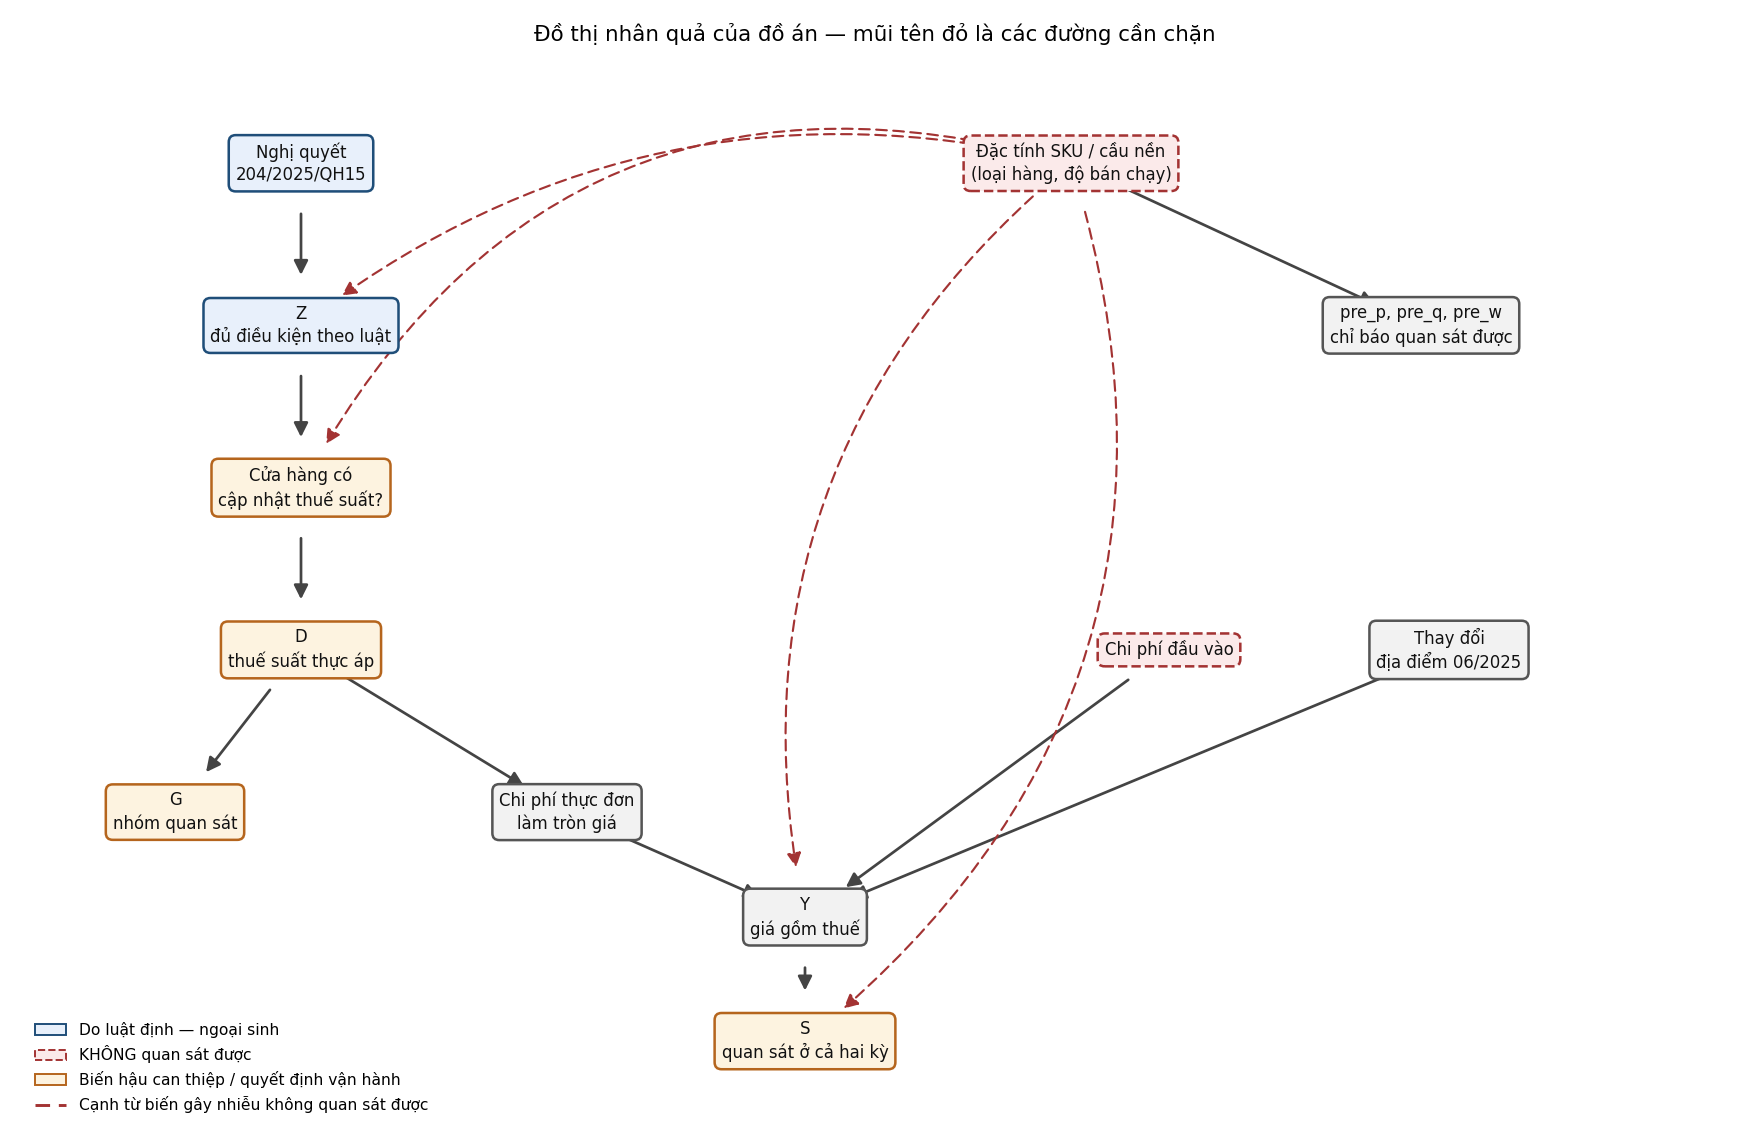
\includegraphics[width=\linewidth]{hinh/do-thi-nhan-qua.png}
  \caption{Đồ thị nhân quả của đồ án. Mũi tên liền là quan hệ đo được từ hóa đơn; mũi tên đứt màu
  đỏ xuất phát từ những yếu tố dữ liệu này không quan sát được. Chính các mũi tên đỏ là lý do đồ án
  chỉ trình bày kết quả như một so sánh có điều chỉnh.}
  \label{fig:dag}
\end{figure}

Bốn đường phải đọc được từ hình~\ref{fig:dag}:

\begin{table}[htbp]
  \centering
  \caption{Bốn đường quan trọng trong đồ thị nhân quả.}
  \label{tab:bon-duong}
  \begin{tabular}{p{5.4cm}p{8.6cm}}
    \toprule
    Đường & Ý nghĩa \\
    \midrule
    Đặc tính SKU $\to Z$
    & Nghị quyết \emph{không tự tạo ra} $Z$. Nghị quyết kết hợp với loại sản phẩm mới xác định đủ
      điều kiện. Một đồ thị chỉ có NQ $\to Z$ sẽ làm can thiệp trông ngoại sinh hơn thực tế. \\
    \addlinespace
    $Z \to$ cửa hàng không cập nhật $\to D \to$ nhóm quan sát
    & Cơ chế làm ô nhiễm nhóm đối chứng nếu chia nhóm theo $D$. \\
    \addlinespace
    Đặc tính SKU $\to$ biến nền, và $\to Y$
    & Cùng một nguyên nhân ẩn vừa gây mất cân bằng, vừa ảnh hưởng xu hướng giá phản thực. Đây là
      đường nguy hiểm nhất. \\
    \addlinespace
    Đặc tính SKU $\to S \leftarrow Y$
    & Collider. Mẫu chỉ giữ SKU có mặt ở cả hai kỳ, mà điều đó lại phụ thuộc chính giá. \\
    \bottomrule
  \end{tabular}
\end{table}

\paragraph{Đường backdoor và khả năng chặn.} Một \emph{đường backdoor} là đường gây nhiễu nối can
thiệp với kết quả mà không đi qua tác động cần đo. Bảng~\ref{tab:backdoor} liệt kê các đường và
trạng thái xử lý.

\begin{table}[htbp]
  \centering
  \caption{Các đường backdoor và cách xử lý.}
  \label{tab:backdoor}
  \begin{tabular}{p{4.6cm}p{4.2cm}p{5.2cm}}
    \toprule
    Đường & Chặn bằng & Trạng thái \\
    \midrule
    $Z \leftarrow$ đặc tính SKU $\to Y$ & Ba biến nền quan sát được
    & Chặn không hoàn toàn --- chúng chỉ là chỉ báo, không phải biến ẩn \\
    \addlinespace
    $D \leftarrow$ cửa hàng cập nhật $\to Y$ & ---
    & Không chặn được. Lý do dùng $Z$ thay vì $D$ \\
    \addlinespace
    $Y \leftarrow$ chi phí đầu vào & ---
    & Không quan sát được. Hóa đơn mua vào chỉ có 03--04/2025 \\
    \addlinespace
    $Y \leftarrow$ thay đổi địa điểm & Cửa sổ từ 11/06 gồm cả hai địa chỉ
    & Giảm nhẹ, không loại bỏ \\
    \addlinespace
    Điều kiện hóa trên $S$ & ---
    & Không sửa được bằng dữ liệu này \\
    \bottomrule
  \end{tabular}
\end{table}

Nguyên tắc bắt buộc: \textbf{không điều chỉnh cho $D$, cho nhóm quan sát, cho $S$, hay bất kỳ biến
nào phát sinh sau can thiệp.}

\subsection{Khung Kết quả tiềm năng}

Ký hiệu phải tách $Z$ và $D$, nếu không thì lý thuyết nói tách nhưng ký hiệu lại gộp:

\begin{table}[htbp]
  \centering
  \caption{Ký hiệu Kết quả tiềm năng.}
  \label{tab:ky-hieu}
  \begin{tabular}{ll}
    \toprule
    Ký hiệu & Nghĩa \\
    \midrule
    $D_i(z)$        & Thuế thực nhận của SKU $i$ nếu trạng thái đủ điều kiện là $z$ \\
    $Y_i(z,d)$      & Thay đổi giá dưới chỉ định $z$ và thuế thực nhận $d$ \\
    $Y_i(1),\,Y_i(0)$ & Dạng rút gọn cho so sánh theo $Z$ \\
    \bottomrule
  \end{tabular}
\end{table}

Chỉ \emph{dưới exclusion restriction} --- $Z$ không ảnh hưởng giá qua kênh nào khác ngoài $D$ ---
mới rút gọn được về $Y_i(d)$.

\paragraph{Vấn đề dữ liệu khuyết.} Với mỗi SKU chỉ quan sát được \emph{một} trong hai kết quả tiềm
năng. Đại lượng $Y_i(0)$ của nhóm đủ điều kiện --- mức đổi giá mà nhóm được giảm thuế lẽ ra có nếu
chính sách không xảy ra --- là thứ \textbf{không bao giờ} quan sát được. Toàn bộ công việc còn lại
của đồ án là dựng một ước lượng cho nó. Đại lượng đích là ATT:
\begin{equation}
  \mathrm{ATT} = \mathbb{E}\big[\,Y_i(1) - Y_i(0)\ \big|\ Z_i = 1\,\big].
  \label{eq:att}
\end{equation}

\paragraph{Lưu ý về tên gọi.} Mẫu đã điều kiện hóa trên việc SKU còn được bán ở cả hai kỳ, mà tỉ
lệ này khác nhau giữa hai nhóm (mục~\ref{sec:song-sot}). Vì vậy đại lượng ước lượng được
\emph{không} phải ITT vô điều kiện cho toàn bộ cohort tiền kỳ, mà là \emph{so sánh theo $Z$ trong
nhóm SKU có giá quan sát được ở cả hai kỳ}.

\subsection{Các giả định và mức độ đáng tin}

\begin{table}[htbp]
  \centering
  \caption{Giả định nhận dạng và đánh giá.}
  \label{tab:gia-dinh}
  \begin{tabular}{p{3.4cm}p{5.0cm}p{5.6cm}}
    \toprule
    Giả định & Nội dung & Đánh giá \\
    \midrule
    Xu hướng song song & Nếu không có chính sách, giá hai nhóm biến động song song
    & Không kiểm chứng được đầy đủ; tiền kỳ quá ngắn \\
    \addlinespace
    Phân loại $Z$ đúng & Định danh sản phẩm phản ánh đúng địa vị pháp lý
    & 23 SKU chưa phân loại được, báo cáo ba biến thể xử lý \\
    \addlinespace
    SUTVA & Không lan tỏa giữa các SKU
    & Đáng ngờ. Khăn ướt và khăn giấy thay thế nhau trong cùng cửa hàng \\
    \addlinespace
    No-anticipation & Cửa hàng không đổi giá trước 01/07 để đón chính sách
    & Kiểm được phần nào bằng giả dược tiền kỳ \\
    \addlinespace
    Ổn định thành phần mẫu & Bộ SKU không đổi hệ thống quanh ngày cắt
    & Có chọn lọc sống sót; xem mục~\ref{sec:song-sot} \\
    \addlinespace
    Không cú sốc trùng thời gian & ---
    & Dữ liệu trống 02--10/06; địa chỉ hóa đơn đổi từ 24/06 \\
    \bottomrule
  \end{tabular}
\end{table}

\subsection{Nghịch lý Simpson và lý do phân tầng}

\emph{Nghịch lý Simpson} là hiện tượng một xu hướng xuất hiện trên toàn mẫu có thể \textbf{đảo
chiều} khi tách theo nhóm nhỏ, do cơ cấu nhóm khác nhau giữa hai bên so sánh. Phân tầng xử lý trực
tiếp hiện tượng này: so sánh \emph{trong từng tầng đồng nhất}, rồi trung bình có trọng số.

Tuy nhiên phân tầng \emph{không tự động} xử lý được Simpson nếu chọn sai biến tầng. Nhóm đã suýt
chọn sai: thiết kế ban đầu định chia tầng theo biến \texttt{type}, cho tới khi phát hiện
\texttt{type} là nhãn cấp \emph{dòng hóa đơn} --- 85\% SKU mang nhiều hơn một nhãn, và ``Ly đá
vừa'' xuất hiện với cả ba nhãn \emph{Nước uống}, \emph{Đồ ăn}, \emph{Sản phẩm khác}.

\subsection{Hai mô hình nhân quả --- và điều chúng không chứng minh được}

Đồ án dùng \textbf{hai mô hình phân tích nhân quả khác nhau} theo yêu cầu đề bài: hồi quy có điều
chỉnh (PP1) và phân tầng theo mức giá (PP2). Nhóm chạy thêm hai biến thể --- PP1-A thô và PP1-B
g-computation --- để so sánh chéo, thành bốn ước lượng.

\begin{quote}
\textbf{Cảnh báo quan trọng.} Cả hai mô hình dùng chung \emph{một} chiến lược nhận dạng: xu hướng
song song. Việc hai phương pháp cho kết quả tương tự \emph{không} xác nhận quan hệ nhân quả --- nếu
giả định chung sai, cả hai cùng sai theo cùng một hướng.
\end{quote}

Dữ liệu này chỉ hỗ trợ một chiến lược nhận dạng: không có ngưỡng hồi quy gián đoạn, và chỉ có một
cửa hàng. Khung Wald dùng $Z$ theo kiểu biến công cụ, nhưng $Z$ chỉ hợp lệ nếu \emph{đã có} xu
hướng song song theo $Z$ --- nó nằm \emph{trong} cùng chiến lược, không độc lập với nó.

% =====================================================================
\section{Bốn cách ước lượng}
\label{sec:bon-cach}
% =====================================================================

\subsection{Đại lượng cần đo}

Với mỗi mặt hàng, lấy giá trung vị trước 01/07 và giá trung vị sau 01/07, rồi tính
\begin{equation}
  Y_i = 100 \times \log\!\left(\frac{P_i^{\text{sau}}}{P_i^{\text{trước}}}\right).
  \label{eq:y}
\end{equation}

Đơn vị gọi là \dvi{}, xấp xỉ phần trăm khi giá trị nhỏ. Dùng log thay vì phần trăm thô vì log
\emph{đối xứng}: tăng rồi giảm cùng một lượng thì về đúng chỗ cũ, còn phần trăm thì không (tăng
10\% rồi giảm 10\% ra 99\%).

\begin{table}[htbp]
  \centering
  \caption{Ví dụ minh họa công thức~\eqref{eq:y}.}
  \label{tab:vi-du-y}
  \begin{tabular}{lrrr}
    \toprule
    Trường hợp & Giá trước & Giá sau & $Y$ \\
    \midrule
    Giữ nguyên giá & 50.000đ & 50.000đ & $0$ \\
    Giảm 1.000đ    & 50.000đ & 49.000đ & $-2{,}02$ \\
    Tăng 2.000đ    & 50.000đ & 52.000đ & $+3{,}92$ \\
    \bottomrule
  \end{tabular}
\end{table}

\subsection{Kết quả đo được: cả hai nhóm đều tăng giá}
\label{sec:mo-ta-y}

\begin{table}[htbp]
  \centering
  \caption{Mô tả biến kết quả theo nhóm, trước mọi phép điều chỉnh. Nguồn:
  \texttt{kq-mo-ta-y-theo-nhom.csv}.}
  \label{tab:mo-ta-y}
  \begin{tabular}{lrr}
    \toprule
    Chỉ số & $Z=1$ (được giảm thuế) & $Z=0$ (đối chứng) \\
    \midrule
    Số mặt hàng          & 155         & 132 \\
    $Y$ trung bình       & $+0{,}624$  & $+1{,}022$ \\
    $Y$ trung vị         & $0{,}000$   & $0{,}000$ \\
    Độ lệch chuẩn        & $6{,}07$    & $3{,}97$ \\
    Giữ nguyên giá y hệt & 126/155     & 103/132 \\
    \bottomrule
  \end{tabular}
\end{table}

Bảng~\ref{tab:mo-ta-y} chứa ba thông tin quyết định cách đọc toàn bộ kết quả về sau:

\begin{enumerate}
  \item \textbf{Không nhóm nào giảm giá.} Cả hai trung bình đều \emph{dương}. Vì vậy chênh lệch
  $-0{,}398$ xuất hiện ở mọi bảng sau là \emph{chênh lệch giữa hai mức tăng}, không phải mức giảm.
  \item \textbf{Trung vị bằng 0 ở cả hai nhóm} --- quá nửa số mặt hàng không đổi giá một đồng nào.
  Toàn bộ biến động nằm ở phần thiểu số còn lại.
  \item \textbf{Nhiễu lớn hơn tín hiệu nhiều lần.} Độ lệch chuẩn $6{,}07$ trong khi đại lượng cần
  đo chỉ cỡ $0{,}4$. Đây là nguyên nhân gốc khiến mọi khoảng tin cậy về sau đều rộng và phủ qua 0.
\end{enumerate}

\subsection{Vì sao không so thẳng được}

\begin{table}[htbp]
  \centering
  \caption{Đặc điểm nền của hai nhóm, đo trước 01/07. Nguồn:
  \texttt{eda-mo-ta-nen-theo-nhom.csv}.}
  \label{tab:bien-nen}
  \begin{tabular}{lrr}
    \toprule
    Đặc điểm nền & $Z=1$ (hóa chất, mỹ phẩm) & $Z=0$ (bia, rượu, thuốc lá) \\
    \midrule
    Giá trung bình            & 72.319đ & 108.913đ \\
    Số lượng bán trung bình   & $6{,}2$ & $33{,}3$ \\
    Số tuần có giao dịch      & $3{,}31$ & $4{,}73$ \\
    \bottomrule
  \end{tabular}
\end{table}

Dòng giữa của bảng~\ref{tab:bien-nen} là dòng quan trọng nhất: \textbf{bia rượu bán gấp hơn năm
lần} hàng hóa chất. Điều này nối thẳng tới hành vi định giá --- món bán chạy thì cửa hàng theo dõi
giá sát và cập nhật thường xuyên theo chi phí đầu vào, còn món bán ế thì giá nằm im hàng tháng.

Nghĩa là kể cả \emph{không có chính sách nào}, hai nhóm này vẫn sẽ có mức đổi giá khác nhau:
\begin{equation}
  \underbrace{-0{,}398}_{\text{chênh lệch đo được}}
  \;=\;
  \underbrace{\text{phần do chính sách}}_{\text{cần ước lượng}}
  \;+\;
  \underbrace{\text{phần do hai nhóm vốn khác nhau}}_{\text{cần trừ đi}}.
  \label{eq:phan-ra-tho}
\end{equation}

Bốn cách ước lượng dưới đây là \textbf{bốn cách trừ phần thứ hai đi}. Chúng khác nhau đúng ở chỗ
đó, không khác ở cách đo $Y$ hay cách chia nhóm.

\begin{figure}[htbp]
  \centering
  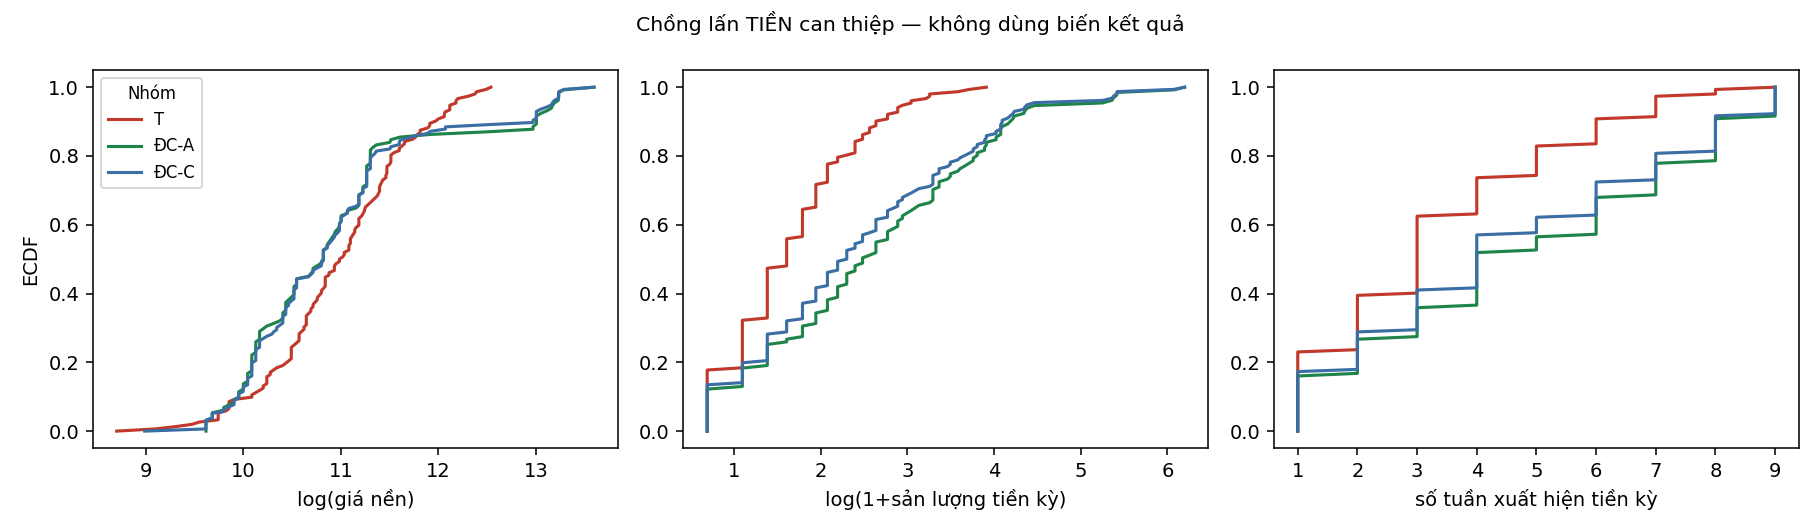
\includegraphics[width=\linewidth]{hinh/eda-chong-lan-tien-ky.png}
  \caption{Chồng lấn ba biến nền giữa nhóm can thiệp và các định nghĩa nhóm đối chứng, đo trên tiền
  kỳ. Hai nhóm lệch nhau rõ ở sản lượng và tần suất bán.}
  \label{fig:chong-lan}
\end{figure}

\subsection{Cách 1 --- Hồi quy thô}

Không điều chỉnh cho khác biệt sẵn có nào:
\begin{equation}
  Y_i = \beta_0 + \beta_1 Z_i + \varepsilon_i.
  \label{eq:pp1a-tho}
\end{equation}

Với $Z$ chỉ nhận giá trị 0 hoặc 1, hồi quy này \emph{đúng bằng} hiệu hai trung bình ở
bảng~\ref{tab:mo-ta-y}:
\[
  \hat\beta_1 = 0{,}6244 - 1{,}0222 = -0{,}3978.
\]

\paragraph{Sai số chuẩn.} Đây là chỗ duy nhất công thức đủ đơn giản để trình bày trực tiếp:
\begin{equation}
  \mathrm{SE}(\hat\beta_1)
  = \sqrt{\frac{s_1^2}{n_1} + \frac{s_0^2}{n_0}}
  = \sqrt{\frac{6{,}070^2}{155} + \frac{3{,}972^2}{132}}
  = 0{,}598.
  \label{eq:se-tho}
\end{equation}
Tử số là độ dao động của $Y$, mẫu số là cỡ mẫu; muốn sai số nhỏ đi một nửa thì cần mẫu gấp bốn.
Sai số chuẩn báo cáo dùng ước lượng vững HC3 ($0{,}600$), không đòi hỏi hai nhóm có cùng phương
sai --- điều cần thiết vì $6{,}07$ và $3{,}97$ lệch nhau rõ.

Cách này lẫn toàn bộ khác biệt sẵn có nên \emph{không} phải câu trả lời. Nó được báo cáo như một
phép đo \textbf{chẩn đoán}: nếu nó và cách có kiểm soát lệch nhau nhiều, đó là bằng chứng các biến
nền đang chi phối.

\subsection{Cách 2 --- Hồi quy có hiệp biến}
\label{sec:cach-2}

Giả định một dạng hàm nối đặc điểm nền với mức đổi giá, cho nó hút phần khác biệt sẵn có; phần còn
lại gán cho $Z$:
\begin{equation}
  Y_i = \beta_0 + \beta_1 Z_i
      + \gamma_1 \log P_i^{\text{nền}}
      + \gamma_2 \log\!\left(1 + Q_i^{\text{nền}}\right)
      + \gamma_3 W_i^{\text{nền}}
      + \varepsilon_i,
  \label{eq:pp1a-hb}
\end{equation}
trong đó $P^{\text{nền}}$ là giá trung vị trước chính sách, $Q^{\text{nền}}$ là số lượng bán trước
chính sách, và $W^{\text{nền}}$ là số tuần có giao dịch trước chính sách.

\begin{table}[htbp]
  \centering
  \caption{Hệ số ước lượng của mô hình~\eqref{eq:pp1a-hb}. Nguồn:
  \texttt{kq-he-so-mo-hinh.csv}.}
  \label{tab:he-so-hb}
  \begin{tabular}{lrl}
    \toprule
    Hệ số & Giá trị & Đọc thế nào \\
    \midrule
    $\beta_0$ (chặn)      & $+0{,}027$ & Mốc xuất phát \\
    $\beta_1$ ($Z$)       & $\mathbf{-0{,}270}$ & \textbf{Con số cần tìm} \\
    $\gamma_1$ (log giá nền)   & $+0{,}097$ & Hàng đắt tăng giá nhỉnh hơn chút \\
    $\gamma_2$ (log sức bán)   & $+0{,}993$ & Bán càng chạy càng tăng giá mạnh \\
    $\gamma_3$ (số tuần bán)   & $-0{,}557$ & Bán càng đều thì giá càng ít nhảy \\
    \bottomrule
  \end{tabular}
\end{table}

Hệ số $\gamma_2 = +0{,}993$ là chỗ đáng chú ý: hàng bán chạy tăng giá mạnh hơn hẳn, mà nhóm đối
chứng bán chạy gấp năm lần (bảng~\ref{tab:bien-nen}). Mô hình dùng đúng thông tin này để trừ bớt
phần ``bia rượu tăng giá vì bia rượu bán chạy'' ra khỏi chênh lệch hai nhóm. Kết quả: từ
$-0{,}398$ thành $-0{,}270$, tức khoảng \textbf{một phần ba} chênh lệch thô đến từ đặc điểm hàng
hóa chứ không từ chính sách.

\paragraph{Một nghịch lý đáng ghi nhận: thêm biến kiểm soát mà sai số tăng.} Sai số chuẩn của
$\hat\beta_1$ tăng từ $0{,}600$ lên $0{,}733$. Nguyên nhân tách bạch được:

\begin{table}[htbp]
  \centering
  \caption{Chẩn đoán tác động của hiệp biến lên sai số. Nguồn:
  \texttt{kq-chan-doan-hiep-bien.csv}.}
  \label{tab:chan-doan-hb}
  \begin{tabular}{lrr}
    \toprule
    Chỉ số & Cách 1 & Cách 2 \\
    \midrule
    Độ lệch chuẩn phần dư          & $5{,}212$ & $5{,}204$ \\
    $R^2$ của mô hình              & $0{,}15\%$ & $1{,}48\%$ \\
    $R^2$ của $Z$ theo $X$         & ---        & $26{,}3\%$ \\
    Sai số chuẩn của $\hat\beta_1$ & $0{,}600$ & $0{,}733$ \\
    \bottomrule
  \end{tabular}
\end{table}

Ba biến nền hầu như \emph{không} giải thích được $Y$ --- phần dư chỉ giảm $0{,}15\%$, nghĩa là mức
đổi giá của một mặt hàng gần như không đoán được từ giá nền, sức bán hay tần suất bán; cửa hàng đổi
giá vì lý do nằm ngoài dữ liệu hóa đơn. Nhưng $Z$ lại \emph{đoán được} từ $X$ tới $26{,}3\%$, vì
hóa chất và bia rượu vốn khác nhau ở đúng ba biến đó. Hệ số phóng đại phương sai
\begin{equation}
  \mathrm{VIF} = \frac{1}{1 - R^2_{Z \sim X}} = \frac{1}{1 - 0{,}263} = 1{,}357,
  \qquad
  0{,}600 \times \sqrt{1{,}357} = 0{,}699 \approx 0{,}733.
  \label{eq:vif}
\end{equation}

Nói gọn: \emph{biến kiểm soát chỉ làm sai số nhỏ đi nếu nó thật sự giải thích được $Y$}. Ở đây nó
không giải thích được gì nhưng lại chồng lấn với $Z$, nên chỉ nhận cái giá mà không nhận cái lợi.

\paragraph{Điểm yếu.} Toàn bộ công thức~\eqref{eq:pp1a-hb} là một \emph{giả định}: nó ép quan hệ
giữa $X$ và $Y$ phải tuyến tính, và ép \emph{cả hai nhóm dùng chung một đường thẳng}. Chính chỗ đó
dẫn tới cách 3.

\subsection{Cách 3 --- g-computation}
\label{sec:cach-3}

Thay vì so hai nhóm trực tiếp, cách này dựng ra \emph{phản thực}: mức đổi giá mà nhóm $Z=1$ lẽ ra
có nếu chính sách không xảy ra. Không quan sát được đại lượng đó, nhưng có thể \emph{học} nó từ
nhóm đối chứng --- nhóm đang sống trong đúng thế giới không có chính sách.

\begin{enumerate}
  \item Khớp mô hình $\hat m_0(X)$ bằng bình phương tối thiểu, \textbf{chỉ trên 132 SKU nhóm
  $Z=0$}, không đụng tới nhóm $Z=1$.
  \item Đưa $X$ của từng SKU trong nhóm $Z=1$ vào $\hat m_0$ để dự đoán mức đổi giá phản thực.
  \item Lấy giá thật trừ giá dự đoán, rồi trung bình trên toàn nhóm $Z=1$.
\end{enumerate}

\begin{equation}
  \widehat{\mathrm{ATT}}
  = \frac{1}{n_1}\sum_{i:\,Z_i = 1} \Big[\, Y_i - \hat m_0(X_i) \,\Big].
  \label{eq:g-comp}
\end{equation}

\begin{table}[htbp]
  \centering
  \caption{Hệ số của $\hat m_0$, khớp chỉ trên nhóm $Z=0$, và phép phân rã dự báo phản thực. Cột
  ``chênh lệch $X$'' là trung bình $X$ nhóm $Z=1$ trừ nhóm $Z=0$. Nguồn:
  \texttt{kq-he-so-mo-hinh.csv}.}
  \label{tab:g-comp}
  \begin{tabular}{lrrr}
    \toprule
    Thành phần & Hệ số & Chênh lệch $X$ & Đóng góp \\
    \midrule
    Trung bình $Y$ nhóm $Z=0$ & --- & --- & $1{,}0222$ \\
    log giá nền     & $-0{,}479$ & $+0{,}0086$ & $-0{,}0041$ \\
    log sức bán     & $+0{,}547$ & $-0{,}9297$ & $-0{,}5085$ \\
    số tuần bán     & $-0{,}546$ & $-1{,}4252$ & $+0{,}7785$ \\
    \midrule
    \textbf{Dự báo phản thực cho nhóm $Z=1$} & & & $\mathbf{1{,}2882}$ \\
    \bottomrule
  \end{tabular}
\end{table}

Từ đó:
\[
  \widehat{\mathrm{ATT}} = 0{,}6244 - 1{,}2882 = -0{,}6638.
\]

\paragraph{Vì sao cách 3 khác cách 2 tới vậy?} Hai cách chỉ khác nhau ở chỗ \emph{tin hệ số của
ai}: khớp trên cả hai nhóm, hay khớp chỉ trên nhóm đối chứng.

\begin{table}[htbp]
  \centering
  \caption{So sánh hệ số hai mô hình và phân rã chênh lệch giữa hai ước lượng.}
  \label{tab:so-he-so}
  \begin{tabular}{lrrrr}
    \toprule
    Hiệp biến & Khớp cả hai nhóm & Khớp chỉ $Z=0$ & Chênh lệch $X$ & Đóng góp vào chênh lệch \\
    \midrule
    log giá nền & $+0{,}097$ & $-0{,}479$ & $+0{,}0086$ & $+0{,}005$ \\
    log sức bán & $+0{,}993$ & $+0{,}547$ & $-0{,}9297$ & $\mathbf{-0{,}414}$ \\
    số tuần bán & $-0{,}557$ & $-0{,}546$ & $-1{,}4252$ & $+0{,}015$ \\
    \midrule
    \textbf{Tổng} & & & & $\mathbf{-0{,}394}$ \\
    \bottomrule
  \end{tabular}
\end{table}

Phép kiểm khớp chính xác: $-0{,}270 - (-0{,}664) = +0{,}394$. Nói cách khác,
\textbf{toàn bộ khoảng cách giữa hai ước lượng nằm ở một biến duy nhất --- sức bán}. Mô hình gộp
nói một đơn vị log sức bán kéo $Y$ lên $0{,}99$; mô hình chỉ học từ bia rượu nói chỉ $0{,}55$. Vì
nhóm $Z=1$ bán ế hơn $0{,}93$ đơn vị log, hai con số đó dẫn tới hai phản thực cách nhau $0{,}39$.

Ai đúng thì dữ liệu trong tay \emph{không phân xử được}: cách 2 đánh cược rằng hai nhóm chung một
quy luật, cách 3 đánh cược rằng quy luật của bia rượu áp được cho hàng hóa chất. Đây chính là bản
chất của giả định, và là lý do đồ án báo cáo cả bốn con số thay vì chọn một.

\paragraph{Điều kiện chồng lấn.} Muốn áp $\hat m_0$ lên nhóm $Z=1$ thì các SKU $Z=1$ phải nằm
trong tầm dữ liệu của nhóm $Z=0$, nếu không mô hình đang \emph{ngoại suy}. Đo được: $2{,}6\%$ SKU
$Z=1$ nằm ngoài khoảng của $Z=0$, toàn bộ ở biến giá nền; sức bán và tần suất chồng lấn hoàn toàn.
Tỉ lệ này đủ nhỏ để dùng được, nhưng phải nêu ra.

Khoảng tin cậy và sai số chuẩn của~\eqref{eq:g-comp} tính bằng bootstrap 5.000 vòng, lấy mẫu lại
độc lập trong từng nhóm.

\subsection{Cách 4 --- Phân tầng theo mức giá}
\label{sec:cach-4}

Ba cách trên đều phải giả định một dạng hàm. Cách này \emph{không} giả định gì: nếu chỉ so những
mặt hàng có giá nền gần nhau thì phần khác biệt do giá tự triệt tiêu.

\paragraph{Vì sao chọn giá nền làm biến tầng.} Phần thuế được giảm tương đương khoảng $1{,}8\%$
giá. Với món 10.000đ, đó là khoảng 182đ --- \emph{nhỏ hơn cả bước giá 1.000đ}, nên việc đổi giá cho
đúng gần như không khả thi. Với món 100.000đ, đó là khoảng 1.818đ, tức gần hai bước giá. Hàng rẻ và
hàng đắt vì thế không phản ứng như nhau, và hai nhóm lại có phân bố giá khác nhau.

Chia 287 SKU thành năm tầng theo phân vị giá trước chính sách, tính hiệu hai nhóm riêng trong từng
tầng, rồi gộp lại:
\begin{equation}
  \hat\tau_{\text{PT}} = \sum_{s=1}^{5} w_s \hat\tau_s,
  \qquad
  \hat\tau_s = \bar Y_{s,Z=1} - \bar Y_{s,Z=0},
  \qquad
  w_s = \frac{n_{s,Z=1}}{\sum_{s'} n_{s',Z=1}}.
  \label{eq:pp2}
\end{equation}

Trọng số dùng \emph{số SKU nhóm $Z=1$} chứ không phải tổng số SKU, vì đại lượng đích là ATT --- tác
động trên chính nhóm được luật cho giảm. Nhóm đối chứng chỉ đóng vai thước đo nên không tham gia
định trọng số.

\begin{table}[htbp]
  \centering
  \caption{Kết quả theo năm tầng giá nền. Nguồn: \texttt{kq-theo-tang.csv}.}
  \label{tab:theo-tang}
  \begin{tabular}{crrrrrr}
    \toprule
    Tầng & Khoảng giá nền & $n_{Z=1}$ & $n_{Z=0}$ & $\hat\tau_s$ & $w_s$ & $w_s\hat\tau_s$ \\
    \midrule
    0 & 9.000 -- 26.000đ    & 19 & 39 & $-0{,}076$ & $0{,}123$ & $-0{,}009$ \\
    1 & 27.000 -- 42.000đ   & 39 & 20 & $+0{,}066$ & $0{,}252$ & $+0{,}017$ \\
    2 & 43.000 -- 62.000đ   & 32 & 24 & $-0{,}256$ & $0{,}206$ & $-0{,}053$ \\
    \textbf{3} & \textbf{64.000 -- 96.000đ} & 31 & 27 & $\mathbf{-1{,}662}$ & $0{,}200$
    & $\mathbf{-0{,}332}$ \\
    4 & 99.000 -- 804.000đ  & 34 & 22 & $+0{,}551$ & $0{,}219$ & $+0{,}121$ \\
    \midrule
    & \textbf{Tổng} & \textbf{155} & \textbf{132} & & $1{,}000$ & $\mathbf{-0{,}257}$ \\
    \bottomrule
  \end{tabular}
\end{table}

\paragraph{Một điểm phải nói thẳng.} Cột cuối bảng~\ref{tab:theo-tang} cho thấy tầng 3 một mình
đóng góp $-0{,}332$ trong khi tổng chỉ $-0{,}257$; bốn tầng còn lại cộng lại ra $+0{,}075$, tức
\emph{dương}. Nếu bỏ tầng 3, ước lượng đổi dấu. Con số $-0{,}257$ vì vậy không phải ``năm tầng cùng
cho thấy một hướng''. Với 31 SKU trong một tầng và độ lệch chuẩn cỡ 6, sai số chuẩn của
$\hat\tau_3$ xấp xỉ $1{,}36$ nên $|t| \approx 1{,}22$ và khoảng tin cậy chứa 0. Nhóm \emph{không}
đào sâu riêng tầng này: tách một tầng ra rồi kể chuyện về nó, sau khi đã xem bảng, là cách chắc
chắn nhất để tự lừa mình.

\paragraph{Sai số chuẩn bằng bootstrap.} Ước lượng~\eqref{eq:pp2} không có công thức đóng, nên
sai số được mô phỏng. Mỗi vòng lặp: bốc lại 155 SKU nhóm $Z=1$ và 132 SKU nhóm $Z=0$ \emph{có hoàn
lại} --- mỗi lần bốc một SKU rồi trả lại vào rổ, nên có SKU trúng nhiều lần và có SKU không trúng
lần nào --- rồi \emph{chia lại năm tầng từ đầu} và tính lại trọng số. Việc chia lại tầng là bắt
buộc: ranh giới tầng cũng là đại lượng ước lượng từ dữ liệu nên cũng phải chịu bất định. Lặp 5.000
vòng, cả 5.000 vòng đều hợp lệ; độ lệch chuẩn của 5.000 kết quả là sai số chuẩn, còn khoảng tin cậy
lấy phân vị $2{,}5\%$ và $97{,}5\%$.

% =====================================================================
\section{Kết quả}
\label{sec:ket-qua}
% =====================================================================

\subsection{Bốn ước lượng chính}

\begin{table}[htbp]
  \centering
  \caption{Bốn ước lượng theo $Z$, đơn vị \dvi{}. Nguồn: \texttt{kq-uoc-luong-chinh.csv}.}
  \label{tab:bon-uoc-luong}
  \begin{tabular}{lrrrl}
    \toprule
    Phương pháp & Ước lượng & SE & $p$ & KTC 95\% \\
    \midrule
    PP1-A thô               & $-0{,}398$ & $0{,}600$ & $0{,}507$ & $[-1{,}573;\ +0{,}778]$ \\
    PP1-A có hiệp biến      & $-0{,}270$ & $0{,}733$ & $0{,}713$ & $[-1{,}707;\ +1{,}168]$ \\
    PP1-B g-computation     & $-0{,}664$ & $0{,}776$ & $0{,}398$ & $[-2{,}197;\ +0{,}836]$ \\
    PP2 phân tầng 5 phân vị & $-0{,}257$ & $0{,}592$ & $0{,}661$ & $[-1{,}414;\ +0{,}911]$ \\
    \bottomrule
  \end{tabular}
\end{table}

\textbf{Cả bốn khoảng tin cậy đều chứa 0.} Dữ liệu không loại trừ được khả năng tác động thật bằng
0. Nhưng điều đó \emph{không} có nghĩa tác động bằng 0: cả bốn khoảng cũng chứa $-1{,}4$, tức mức
chuyển gần hết phần thuế. Dữ liệu đơn giản là không đủ hẹp để phân biệt hai khả năng --- hệ quả
trực tiếp của việc độ lệch chuẩn gấp khoảng 15 lần đại lượng cần đo (mục~\ref{sec:mo-ta-y}).

Phát biểu đúng là \emph{``không bác bỏ được giả thuyết tác động bằng 0''}. Phát biểu
\emph{``tác động bằng 0''} hoặc \emph{``chính sách không có tác động''} là sai.

\subsection{Từ chênh lệch ra tỉ lệ chuyển thuế}
\label{sec:pass-through}

Bốn con số ở bảng~\ref{tab:bon-uoc-luong} khó hình dung, nên được quy về một thang dễ đọc hơn bằng
cách chia cho mốc chuyển hoàn toàn~\eqref{eq:moc-log}:
\begin{equation}
  \widehat{\text{pass-through}} = \frac{\hat\tau}{\tau_{\text{full}}}
  = \frac{\hat\tau}{-1{,}835}.
  \label{eq:pass-through}
\end{equation}

\begin{table}[htbp]
  \centering
  \caption{Tỉ lệ phần giảm thuế đi vào giá.}
  \label{tab:pass-through}
  \begin{tabular}{lrr}
    \toprule
    Phương pháp & Ước lượng & Tỉ lệ chuyển thuế \\
    \midrule
    PP1-A thô           & $-0{,}398$ & 22\% \\
    PP1-A có hiệp biến  & $-0{,}270$ & 15\% \\
    PP1-B g-computation & $-0{,}664$ & 36\% \\
    PP2 phân tầng       & $-0{,}257$ & 14\% \\
    \bottomrule
  \end{tabular}
\end{table}

\paragraph{Cách đọc con số này --- điểm dễ hiểu nhầm nhất của báo cáo.} Gốc so sánh
\emph{không} phải số 0. Nhóm đối chứng cho biết trong cùng hai tháng đó, giá ở cửa hàng này
\emph{đang tăng} $+1{,}022$; đó mới là gốc:
\[
  \begin{array}{rl}
    +1{,}022 & \text{nếu không có chính sách, giá lẽ ra tăng chừng này} \\
    +0{,}624 & \text{thực tế nhóm được giảm thuế chỉ tăng chừng này} \\ \hline
    -0{,}398 & \text{chính sách kéo lại được chừng này} \\[0.3em]
    -1{,}835 & \text{nếu chuyển hết phần thuế, phải kéo được chừng này}
  \end{array}
\]

Do đó \textbf{22\% không có nghĩa là giá giảm 22\%}. Giá vẫn tăng, chỉ tăng ít hơn kịch bản không
có chính sách. Tỉ lệ là phần trăm \emph{của mức lẽ ra kéo được}, không phải phần trăm của giá.

Cần nói thêm ngay: toàn bộ con số này đứng hay sập theo giả định rằng nếu không có chính sách, giá
hàng hóa chất sẽ tăng đúng như bia rượu đã tăng. Giả định đó không kiểm chứng trực tiếp được, và
cổng cân bằng cho thấy nó đáng ngờ.

\subsection{Hai giả thuyết}

\begin{table}[htbp]
  \centering
  \caption{Kiểm định hai giả thuyết. Nguồn: \texttt{kq-uoc-luong-chinh.csv}.}
  \label{tab:hai-gia-thuyet}
  \begin{tabular}{lrll}
    \toprule
    Phương pháp & Pass-through & $H_0$: ATT $=0$ & $H_0$: chuyển hoàn toàn \\
    \midrule
    PP1-A thô           & $+0{,}217$ & $p = 0{,}507$ & $p = 0{,}017$ $\to$ bác bỏ \\
    PP1-A có hiệp biến  & $+0{,}147$ & $p = 0{,}713$ & $p = 0{,}033$ $\to$ bác bỏ \\
    \textbf{PP1-B g-computation} & $+0{,}362$ & $p = 0{,}397$
    & $\mathbf{p = 0{,}131 \to}$ \textbf{KHÔNG bác bỏ} \\
    PP2 phân tầng       & $+0{,}140$ & $p = 0{,}661$ & $p = 0{,}008$ $\to$ bác bỏ \\
    \bottomrule
  \end{tabular}
\end{table}

\begin{quote}
\textbf{Việc bác bỏ mốc chuyển hoàn toàn phụ thuộc phương pháp.} Ba đặc tả bác bỏ, g-computation
không. Theo quy tắc khóa trước khi chạy, \emph{không} lấy tỉ số ``ba trên bốn'' làm biểu quyết. Các
ước lượng điểm đều gần 0 hơn mốc chuyển hoàn toàn, nhưng việc bác bỏ mốc đó là một
\emph{kết quả nhạy với mô hình}.
\end{quote}

Nguyên nhân g-computation lệch: nó vừa cho ước lượng xa 0 nhất ($-0{,}664$, tức tỉ lệ chuyển thuế
cao nhất 36\%) vừa có sai số lớn nhất ($0{,}776$). Khoảng cách từ $-0{,}664$ tới $-1{,}835$ chỉ là
$1{,}17$ sai số chuẩn, trong khi với PP2 khoảng cách đó là $2{,}66$.

\subsection{Ba cổng chẩn đoán}
\label{sec:ba-cong}

Ba tiêu chí được khóa \emph{trước} khi chạy phân tích, để tránh việc chọn tiêu chí sau khi đã thấy
kết quả.

\begin{table}[htbp]
  \centering
  \caption{Ba cổng chẩn đoán và kết quả. Nguồn: \texttt{kq-cong-chan-doan.csv},
  \texttt{kq-smd-sau-phan-tang.csv}.}
  \label{tab:ba-cong}
  \begin{tabular}{p{4.2cm}p{4.6cm}p{5.0cm}}
    \toprule
    Cổng & Tiêu chí khóa trước & Kết quả \\
    \midrule
    1 --- Cân bằng sau phân tầng & $\le 1/3$ số cặp có $|\mathrm{SMD}| > 0{,}25$
    & \textbf{TRƯỢT} --- 12/15 cặp vượt ngưỡng \\
    \addlinespace
    2 --- Giả dược 05 $\to$ 06 & $|\hat\tau| \le 0{,}918$
    & \textbf{ĐẠT} --- lớn nhất $0{,}562$ \\
    \addlinespace
    3 --- TOST tiền xu hướng & $p < 0{,}05$ ở biên $\pm 0{,}918$
    & \textbf{KHÔNG ĐẠT} --- $p$ từ $0{,}090$ đến $0{,}244$ \\
    \bottomrule
  \end{tabular}
\end{table}

Giả dược cho so sánh chính theo $Z$ cho $-0{,}195$ (thô) và $+0{,}101$ (có hiệp biến), đều nhỏ hơn
ngưỡng. Hiệp biến của giả dược được tính \emph{lại chỉ trên tháng 05}; dùng biến nền của đặc tả
chính sẽ là rò rỉ, vì chúng tính trên 05+06 mà tháng 06 chính là kỳ ``hậu'' của giả dược.

\begin{quote}
\textbf{Ba cổng không phải ba lá phiếu.} Cổng 2 đạt \emph{không bù} được cổng 1 và cổng 3. Không
phát hiện chênh lệch giả dược vượt ngưỡng định trước, nhưng kiểm định tương đương không đạt và mất
cân bằng tiền kỳ còn nghiêm trọng. Giả định xu hướng song song \textbf{không được xác nhận}; mọi
diễn giải nhân quả trong báo cáo này chỉ có điều kiện.
\end{quote}

Đã thử \emph{sáu} phương án chia tầng khác --- theo sản lượng, theo số tuần, theo điểm tổng hợp,
theo lưới hai chiều --- và không phương án nào đạt cân bằng. Đây là đặc điểm thật của dữ liệu chứ
không phải lỗi kỹ thuật: rượu bia và hàng chăm sóc cá nhân khác nhau về bản chất luân chuyển, và
không cách chia tầng nào theo biến quan sát được làm chúng giống nhau.

\subsection{Đối chiếu cơ học: giá có rơi đúng mức phải có không?}
\label{sec:bam-chuan}

Mọi kết quả ở trên đều phụ thuộc vào nhóm đối chứng và giả định xu hướng song song. Mục này trả lời
một câu hỏi \emph{khác}, bằng một phép tính \emph{không cần giả định nhận dạng nào}:

\begin{quote}
Nếu cửa hàng thật sự giảm giá theo phần thuế được giảm, giá mới của từng mặt hàng phải là bao
nhiêu --- và giá thực tế có rơi đúng vào đó không?
\end{quote}

\begin{equation}
  B_i = \mathrm{round}_{1000}\!\left( P_i^{\text{trước}} \times \frac{1{,}08}{1{,}10} \right),
  \qquad
  \text{gọi là \emph{bám chuẩn} nếu } \big|P_i^{\text{sau}} - B_i\big| < 1\ \text{đồng}.
  \label{eq:bam-chuan}
\end{equation}

\begin{table}[htbp]
  \centering
  \caption{Đối chiếu giá thực tế với chuẩn cơ học. Khoảng tin cậy dùng phương pháp Wilson --- công
  thức Wald sụp về $[0;0]$ khi tử số nhỏ như ở đây. Nguồn: \texttt{kq-bam-chuan-co-hoc.csv}.}
  \label{tab:bam-chuan}
  \begin{tabular}{lrrrl}
    \toprule
    Nhóm & Lẽ ra phải đổi giá & Bám chuẩn & Tỉ lệ & KTC 95\% \\
    \midrule
    Được giảm thuế ($Z=1$)          & \textbf{135} & \textbf{1} & \textbf{0,7\%} & $[0{,}1\%;\ 4{,}1\%]$ \\
    Đối chiếu, không được giảm ($Z=0$) & 92 & 1 & 1,1\% & $[0{,}2\%;\ 5{,}9\%]$ \\
    \bottomrule
  \end{tabular}
\end{table}

Trong 135 mặt hàng được giảm thuế mà lẽ ra phải đổi giá, chỉ \textbf{1} mặt hàng đạt đúng mức dự
kiến, và \textbf{110} mặt hàng vẫn giữ nguyên giá cũ. Tỉ lệ bám chuẩn ở nhóm được giảm thuế cũng
\emph{không cao hơn} nhóm đối chiếu --- nhóm vốn không được giảm thuế nên mức ``dự kiến'' với chúng
chỉ là một con số giả định. Vì vậy vài lần giá tình cờ trùng mức dự kiến không tạo thành dấu hiệu
cho thấy cửa hàng đã điều chỉnh giá theo thuế.

Ngoài ra, mô phỏng cho thấy riêng cơ chế \emph{làm tròn} không giải thích được việc giá đứng im:
với lưới 1.000đ thì 135/155 SKU vẫn buộc phải đổi mức giá, với lưới 500đ là 152/155 và với lưới
100đ là toàn bộ 155/155.

\begin{quote}
\textbf{Lưu ý về vai trò.} Đây là \emph{so sánh mô tả với một mức giá giả định}, không phải ước
lượng tác động nhân quả. Nó trả lời ``giá có bám mức đó không'', không trả lời ``chính sách gây ra
điều gì''. Phân tích này được bổ sung \emph{sau khi} đã xem kết quả chính, và điều đó được ghi nhận
minh bạch.
\end{quote}

\subsection{Hai cách đọc kết quả}

Hai con số trung tâm của báo cáo trả lời hai câu hỏi khác nhau, và mỗi cái mạnh ở chỗ cái kia yếu.

\begin{table}[htbp]
  \centering
  \caption{Hai cách đọc kết quả.}
  \label{tab:hai-cach-doc}
  \begin{tabular}{p{3.0cm}p{4.6cm}p{2.4cm}p{4.0cm}}
    \toprule
    & Câu hỏi nó trả lời & Kết quả & Cần giả định gì \\
    \midrule
    Tỉ lệ chuyển thuế & So với kịch bản không có chính sách, giá thấp hơn được bao nhiêu?
    & 14\% -- 36\% mức lẽ ra & Xu hướng song song --- cổng cân bằng đã trượt \\
    \addlinespace
    Bám chuẩn cơ học & Giá có rơi đúng con số số học phải có không?
    & 1/135 mặt hàng & Không cần giả định nào \\
    \bottomrule
  \end{tabular}
\end{table}

Tỉ lệ chuyển thuế là ước lượng nhân quả, nhưng thừa hưởng toàn bộ bất định của giả định xu hướng
song song, và khoảng tin cậy của cả bốn cách đều phủ qua 0. Bám chuẩn cơ học không cần giả định
nào, nhưng chỉ mô tả --- nó không nói được nguyên nhân, chỉ nói giá đã không rơi vào con số số học
đáng lẽ phải có. Đặt cạnh nhau, chúng là hai chân của cùng một kết luận.

\subsection{Kết quả phụ và độ nhạy}

\paragraph{Giá chưa thuế.} Giá chưa thuế \emph{tăng} $+1{,}286$ \dvi{} ($p = 0{,}082$); với đặc tả
per-protocol thì $+1{,}515$ ($p = 0{,}036$). Hướng này phù hợp với việc doanh thu chưa thuế của cửa
hàng tăng khi thuế suất giảm mà giá gồm thuế giữ nguyên. Tuy nhiên \textbf{không được} phát biểu
thành ``cửa hàng giữ lại phần giảm thuế'': dữ liệu không có chi phí đầu vào nên không nói được gì
về biên lợi nhuận.

\paragraph{Per-protocol theo $D$.} So sánh theo thuế cửa hàng thực áp cần thêm giả định rằng quyết
định cập nhật thuế không liên quan xu hướng giá phản thực, nên chỉ là kết quả phụ:

\begin{table}[htbp]
  \centering
  \caption{Kết quả per-protocol theo $D$ với các định nghĩa nhóm đối chứng khác nhau.}
  \label{tab:per-protocol}
  \begin{tabular}{lrrr}
    \toprule
    Nhóm đối chứng & $n_0$ & Ước lượng & $p$ \\
    \midrule
    ĐC-A rượu, bia, thuốc lá & 132 & $-0{,}264$ & $0{,}714$ \\
    ĐC-B bỏ hàng hóa chất    & 137 & $-0{,}203$ & $0{,}769$ \\
    ĐC-C đầy đủ              & 157 & $-0{,}076$ & $0{,}903$ \\
    ĐC-8\% (độ nhạy)         & 1.908 & $+0{,}927$ & $0{,}134$ \\
    \bottomrule
  \end{tabular}
\end{table}

\paragraph{Độ nhạy theo cửa sổ thời gian.} Kết luận ổn định qua bốn cửa sổ:

\begin{table}[htbp]
  \centering
  \caption{Độ nhạy theo cửa sổ thời gian. Nguồn: \texttt{kq-do-nhay.csv}.}
  \label{tab:do-nhay-cua-so}
  \begin{tabular}{lrrr}
    \toprule
    Cửa sổ & $n$ & Ước lượng theo $Z$ & $p$ \\
    \midrule
    Chính (05+06 $\to$ 07+08)         & 287 & $-0{,}270$ & $0{,}713$ \\
    Có tháng 4                        & 293 & $-0{,}113$ & $0{,}876$ \\
    Hẹp một tháng (06 $\to$ 07)       & 251 & $-0{,}214$ & $0{,}782$ \\
    Từ 11/06 (gồm cả hai địa chỉ)     & 248 & $-0{,}212$ & $0{,}790$ \\
    \bottomrule
  \end{tabular}
\end{table}

Kết luận cũng ổn định qua ba cách xử lý 23 SKU chưa phân loại được ($-0{,}270$ khi loại,
$-0{,}334$ khi gán tất cả $Z=1$, $-0{,}109$ khi gán tất cả $Z=0$) và hai cách xử lý 9 SKU hòa VAT.
Riêng khi nâng ngưỡng số tuần xuất hiện lên $\ge 5$, ước lượng đổi dấu thành $+0{,}875$ --- nhưng
lúc đó $n$ chỉ còn 104 và khoảng tin cậy rất rộng $[-0{,}75;\ +2{,}50]$.

% =====================================================================
\section{Độ chắc chắn và phạm vi áp dụng}
% =====================================================================

\subsection{Độ lớn tối thiểu phát hiện được}

MDE (Minimum Detectable Effect) là độ lớn tác động nhỏ nhất mà thiết kế có thể phát hiện với sức
mạnh 80\% ở mức ý nghĩa 5\%:
\begin{equation}
  \mathrm{MDE} = \left(z_{1-\alpha/2} + z_{0{,}80}\right) \times \mathrm{SE}
               \approx 2{,}802 \times \mathrm{SE}.
  \label{eq:mde}
\end{equation}

\begin{table}[htbp]
  \centering
  \caption{MDE và sức mạnh tại mốc chuyển hoàn toàn. Nguồn: \texttt{kq-mde-va-suc-manh.csv}.}
  \label{tab:mde}
  \begin{tabular}{lrrr}
    \toprule
    Đặc tả & SE & MDE & Sức mạnh tại $\tau_{\text{full}}$ \\
    \midrule
    PP1-A thô           & $0{,}600$ & $1{,}680$ & 86\% \\
    PP1-A có hiệp biến  & $0{,}733$ & $2{,}055$ & 71\% \\
    PP1-B g-computation & $0{,}776$ & $2{,}173$ & 66\% \\
    PP2 phân tầng       & $0{,}592$ & $1{,}660$ & 87\% \\
    \bottomrule
  \end{tabular}
\end{table}

MDE nằm trong khoảng $1{,}66$--$2{,}17$ \dvi{}. Thiết kế đủ sức phát hiện mức chuyển hoàn toàn
($1{,}835$) ở PP1-A thô và PP2, nhưng chưa đủ ở hai đặc tả còn lại --- đây là lý do kết luận về
chuyển hoàn toàn phụ thuộc phương pháp. Mô phỏng tái định tâm cho MDE khoảng $2{,}10$, gần với kết
quả giải tích $2{,}05$, xác nhận cách tính hoạt động đúng.

\paragraph{Sức mạnh của kiểm định tương đương.} Sức mạnh TOST ở biên đang dùng là \textbf{0,0\%}
trong cả bốn đặc tả. Vì vậy việc TOST thất bại \emph{không phải} bằng chứng chống lại sự tương
đương; thiết kế đơn giản là chưa đủ chính xác cho biên này. Không được suy từ ``TOST thất bại'' ra
``pass-through khác 0''.

\subsection{Chọn lọc sống sót}
\label{sec:song-sot}

Giá hậu kỳ chỉ quan sát được khi SKU còn được bán. Tỉ lệ còn bán ở hậu kỳ là 82,0\% với nhóm $Z=1$
($n = 189$) và 89,2\% với nhóm $Z=0$ ($n = 148$) --- chênh \textbf{7,2 điểm phần trăm}.

Vì mẫu đã điều kiện hóa trên một biến hậu can thiệp, kết quả chính là so sánh theo $Z$
\emph{trong nhóm SKU có giá quan sát được ở cả hai kỳ}, không đại diện cho toàn bộ cohort tiền kỳ.
Đây chính là đường collider trong bảng~\ref{tab:bon-duong}, và nó không sửa được bằng dữ liệu này.

\subsection{Nhánh sản lượng --- khám phá}

Chênh lệch sản lượng ước lượng là $-20{,}6$ \dvi{} ($p = 0{,}067$), nhưng MDE của nhánh này là
\textbf{31,5} điểm và mẫu vẫn chịu chọn lọc sống sót. Thiết kế không đủ lực để kết luận, nên kết
quả này chỉ dùng để khám phá và \emph{không} được gọi là tác động chính sách. Giá trị $p = 0{,}067$
cũng không được diễn giải thành ``suýt có ý nghĩa'' --- $p$ không có ngưỡng ``suýt''.

\subsection{Phạm vi của bất định}

HC3 và bootstrap chỉ đo bất định \emph{giữa các SKU trong mẫu} --- tức trả lời câu hỏi ``nếu cửa
hàng có tập mặt hàng khác đi một chút thì con số nhảy cỡ nào''. Chúng \emph{không} đo:

\begin{itemize}
  \item liệu nhóm bia rượu có phải nhóm đối chứng hợp lệ hay không (cổng cân bằng đã trượt);
  \item liệu việc phân loại $Z$ theo tên hàng có đúng hay không;
  \item liệu một cửa hàng có đại diện cho điều gì rộng hơn hay không.
\end{itemize}

Đặc biệt, dù có 287 hay 287.000 mặt hàng thì vẫn chỉ có \emph{một} chính sách áp \emph{một} lần ở
\emph{một} cửa hàng. Bất định ở cấp chính sách không ước lượng được bằng dữ liệu này. Nói gọn: sai
số $\pm 0{,}6$ là bất định về việc mẫu rơi vào những mặt hàng nào, không phải bất định về việc kết
luận có đúng hay không --- loại thứ hai lớn hơn nhiều và không có con số nào diễn tả được.

% =====================================================================
\section{Thảo luận}
% =====================================================================

\subsection{Những gì đứng vững}

\begin{itemize}
  \item Trong 155 SKU đủ điều kiện đã phân loại, cửa hàng cập nhật thuế suất cho 135 và không cập
  nhật cho 20. Không tuân thủ là hiện tượng \emph{quan sát được}, không phải suy đoán.
  \item Nhóm đủ điều kiện bán ít và thưa hơn rõ rệt so với nhóm thuế tiêu thụ đặc biệt; điều chỉnh
  theo năm phân vị giá \emph{không} tạo được cân bằng cục bộ.
  \item Chênh lệch quan sát dao động trong khoảng $-0{,}11$ đến $-0{,}66$ \dvi{} tùy phương pháp và
  biến thể, và \emph{mọi} khoảng tin cậy đều chứa 0.
  \item Kết luận ổn định qua bốn cửa sổ thời gian, ba cách xử lý SKU chưa phân loại, và hai cách xử
  lý SKU hòa VAT.
  \item Chỉ 1 trên 135 mặt hàng lẽ ra phải đổi giá rơi đúng mức chuẩn cơ học, và 110 mặt hàng giữ
  nguyên giá cũ --- phép đếm này không cần giả định nhận dạng nào.
\end{itemize}

\subsection{Những gì không được kết luận}

Bảng~\ref{tab:cau-cam} liệt kê các phát biểu bị loại trừ và lý do. Danh sách này được khóa trước
khi chạy phân tích và được một script rà soát tự động kiểm tra trên toàn bộ sản phẩm nộp.

\begin{table}[htbp]
  \centering
  \caption{Các phát biểu không được viết, và lý do.}
  \label{tab:cau-cam}
  \begin{tabular}{p{6.4cm}p{7.6cm}}
    \toprule
    Phát biểu bị loại trừ & Vì sao \\
    \midrule
    ``Chính sách không có tác động'' / ``tác động bằng 0''
    & Không bác bỏ được $\ne$ bằng 0. TOST thất bại ở mọi biên \\
    \addlinespace
    ``Cửa hàng giữ lại phần giảm thuế''
    & Không có dữ liệu chi phí đầu vào để nói về biên lợi nhuận \\
    \addlinespace
    ``Bác bỏ chuyển hoàn toàn'' như kết luận chính
    & Phụ thuộc phương pháp --- g-computation không bác bỏ \\
    \addlinespace
    ``Hai phương pháp xác nhận lẫn nhau''
    & Cả hai dùng chung một chiến lược nhận dạng \\
    \addlinespace
    ``Xu hướng song song đã được chứng minh''
    & Cổng 3 không đạt, cổng 1 trượt \\
    \addlinespace
    Ngoại suy ra cửa hàng khác hoặc toàn ngành
    & Một cửa hàng, một ngày chính sách \\
    \addlinespace
    Gọi kết quả là ITT mà không kèm điều kiện mẫu
    & Mẫu đã điều kiện hóa sống sót, chênh 7,2 điểm phần trăm \\
    \bottomrule
  \end{tabular}
\end{table}

\subsection{Hạn chế}

\paragraph{Chi phí đổi giá.} Cửa hàng có thể ngại đổi giá vì mỗi lần đổi đều tốn công và ảnh hưởng
vận hành. Dữ liệu hóa đơn không quan sát được chi phí này, nên đồ án không tách được phần do ngại
đổi giá khỏi phần do chính sách.

\paragraph{Lạm phát tích lũy.} Phần giảm thuế có thể đã bị phần lạm phát tích lũy từ lần điều chỉnh
giá gần nhất bù vào. Dữ liệu không quan sát được chi phí đầu vào, nên đây là khả năng chưa loại trừ
được.

\paragraph{Hai nhóm khác nhau từ trước.} Hàng hóa chất bán chậm hơn hẳn bia rượu, và không phương án
phân tầng nào theo biến quan sát được khắc phục được điều đó. Vì vậy chưa xác định được chính xác
bao nhiêu phần chênh lệch là do chính sách.

\subsection{Hướng mở rộng}

\begin{itemize}
  \item \textbf{Nhiều cửa hàng.} Có dữ liệu từ nhiều cửa hàng sẽ cho phép ước lượng bất định ở cấp
  chính sách và kiểm tra tính khái quát.
  \item \textbf{Dữ liệu chi phí đầu vào.} Có hóa đơn mua vào ở cả hai kỳ sẽ cho phép tách phần lạm
  phát chi phí khỏi phần chính sách, và trả lời được câu hỏi về biên lợi nhuận.
  \item \textbf{Tiền kỳ dài hơn.} Chuỗi giá dài trước chính sách sẽ cho phép kiểm chứng xu hướng
  song song bằng nhiều hệ số dẫn, thay vì chỉ hai như hiện nay.
\end{itemize}

% =====================================================================
\section{Kết luận}
% =====================================================================

Kết quả rõ nhất của đồ án là \textbf{cửa hàng đã không chuyển hết phần giảm thuế GTGT vào giá bán
lẻ}.

Nếu cửa hàng giảm giá đúng theo phần thuế được giảm và làm tròn đến 1.000 đồng, 135 mặt hàng lẽ ra
phải đổi giá. Thực tế chỉ \textbf{1} mặt hàng đạt đúng mức đó, còn \textbf{110} mặt hàng giữ nguyên
giá cũ. Phép đếm này thuần số học trên hóa đơn, không cần nhóm đối chứng và không cần giả định nhận
dạng nào.

Bốn cách ước lượng nhân quả cho tỉ lệ chuyển thuế vào giá chỉ khoảng \textbf{14\%--36\%} mức lẽ ra
phải đạt. Cả bốn đều cùng chiều, nhưng khoảng tin cậy đều phủ qua 0, nên các con số này chưa đủ
chính xác để nói tỉ lệ thật là bao nhiêu.

Giá trung bình nhóm được giảm thuế tăng khoảng $0{,}6\%$, nhóm không được giảm tăng khoảng
$1{,}0\%$. Có khả năng chính sách đã giúp nhóm được giảm thuế tăng giá ít hơn, nhưng ba cổng chẩn
đoán cho thấy dữ liệu chưa đủ mạnh để xác định bao nhiêu phần chênh lệch này là do chính sách. Điều
đó giới hạn \emph{độ lớn} của tác động ước lượng được, \emph{không} lật ngược phát hiện quan sát
được rằng giá thực tế đã không giảm theo phần thuế được giảm.

Kết luận áp dụng cho các mặt hàng còn được bán ở \emph{cả hai} giai đoạn, tại \emph{một} cửa hàng
tiện lợi TP.HCM, tiền kỳ 05--06/2025 và hậu kỳ 07--08/2025.

Đóng góp của đồ án nằm ở hai chỗ: đo được mức độ thực thi chính sách ở cấp cửa hàng bằng dữ liệu
giao dịch thật, và cho thấy rõ giới hạn của thiết kế thí nghiệm tự nhiên khi dữ liệu chỉ đến từ một
đơn vị --- bao gồm cả việc trình bày trung thực những cổng chẩn đoán mà đồ án đã không vượt qua.

% =====================================================================
\appendix
\section{Phụ lục: tái lập kết quả}
% =====================================================================

Toàn bộ kết quả trong báo cáo sinh ra từ một lệnh duy nhất:

\begin{verbatim}
python code/chay_tat_ca.py
\end{verbatim}

Pipeline gồm sáu bước: đọc dữ liệu thô, làm sạch và lọc, dựng mẫu, thống kê mô tả, ước lượng, và
suy diễn. Mỗi lần chạy ghi ra \texttt{ket-qua/manifest-tai-lap.json} chứa hash SHA-256 của file
nguồn, phiên bản Python và các thư viện, tham số phân tích (ngày chính sách, cửa sổ, seed, số lần
bootstrap), cùng hash và số dòng của từng file đầu ra. Chạy hai lần cho kết quả hash giống hệt nhau,
kể cả các bảng dùng bootstrap 5.000 vòng.

\begin{table}[htbp]
  \centering
  \caption{Các file kết quả được trích dẫn trong báo cáo.}
  \label{tab:file-ket-qua}
  \begin{tabular}{ll}
    \toprule
    File & Nội dung \\
    \midrule
    \texttt{kq-uoc-luong-chinh.csv}      & Bốn ước lượng, SE, KTC, pass-through \\
    \texttt{kq-theo-tang.csv}            & Kết quả năm tầng và trọng số \\
    \texttt{kq-he-so-mo-hinh.csv}        & Hệ số ba mô hình, chênh lệch hiệp biến \\
    \texttt{kq-chan-doan-hiep-bien.csv}  & Phần dư, $R^2$, VIF \\
    \texttt{kq-mo-ta-y-theo-nhom.csv}    & Mô tả biến kết quả theo nhóm \\
    \texttt{kq-cong-chan-doan.csv}       & Giả dược và TOST tiền xu hướng \\
    \texttt{kq-smd-sau-phan-tang.csv}    & SMD từng biến trong từng tầng \\
    \texttt{kq-bam-chuan-co-hoc.csv}     & Đối chiếu chuẩn cơ học \\
    \texttt{kq-mde-va-suc-manh.csv}      & MDE và đường cong sức mạnh \\
    \texttt{kq-do-nhay.csv}              & Lưới độ nhạy đầy đủ \\
    \texttt{eda-mo-ta-nen-theo-nhom.csv} & Ba biến nền theo nhóm \\
    \texttt{eda-ma-tran-chuyen-thue.csv} & Ma trận chuyển thuế suất \\
    \bottomrule
  \end{tabular}
\end{table}

Ngoài báo cáo này, kết quả còn được trình bày dưới hai dạng khác, cả hai đều \emph{đọc thẳng} từ
các file trên nên không thể lệch khỏi phân tích:

\begin{itemize}
  \item \textbf{Web} --- ứng dụng FastAPI + Next.js với 7 trang phân tích và 5 biểu đồ.
  \item \textbf{Bộ trình chiếu} --- 25 slide tại đường dẫn \texttt{/trinh-bay} của cùng ứng dụng.
\end{itemize}

% =====================================================================
\begin{thebibliography}{9}

\bibitem{nq204}
Quốc hội nước Cộng hòa xã hội chủ nghĩa Việt Nam.
\newblock Nghị quyết số 204/2025/QH15 về giảm thuế giá trị gia tăng.
\newblock Hiệu lực từ 01/07/2025.

\bibitem{nq174}
Quốc hội nước Cộng hòa xã hội chủ nghĩa Việt Nam.
\newblock Nghị quyết số 174/2024/QH15 về giảm thuế giá trị gia tăng.
\newblock Hiệu lực đến 30/06/2025.

\bibitem{pearl2009}
Judea Pearl.
\newblock \textit{Causality: Models, Reasoning and Inference}.
\newblock Cambridge University Press, ấn bản thứ hai, 2009.

\bibitem{imbens2015}
Guido W. Imbens and Donald B. Rubin.
\newblock \textit{Causal Inference for Statistics, Social, and Biomedical Sciences: An
Introduction}.
\newblock Cambridge University Press, 2015.

\bibitem{angrist2009}
Joshua D. Angrist and Jörn-Steffen Pischke.
\newblock \textit{Mostly Harmless Econometrics: An Empiricist's Companion}.
\newblock Princeton University Press, 2009.

\bibitem{robins1986}
James M. Robins.
\newblock A new approach to causal inference in mortality studies with a sustained exposure period.
\newblock \textit{Mathematical Modelling}, 7(9--12):1393--1512, 1986.

\bibitem{mackinnon1985}
James G. MacKinnon and Halbert White.
\newblock Some heteroskedasticity-consistent covariance matrix estimators with improved finite
sample properties.
\newblock \textit{Journal of Econometrics}, 29(3):305--325, 1985.

\bibitem{efron1979}
Bradley Efron.
\newblock Bootstrap methods: Another look at the jackknife.
\newblock \textit{The Annals of Statistics}, 7(1):1--26, 1979.

\bibitem{wilson1927}
Edwin B. Wilson.
\newblock Probable inference, the law of succession, and statistical inference.
\newblock \textit{Journal of the American Statistical Association}, 22(158):209--212, 1927.

\bibitem{lakens2017}
Daniël Lakens.
\newblock Equivalence tests: A practical primer for $t$-tests, correlations, and meta-analyses.
\newblock \textit{Social Psychological and Personality Science}, 8(4):355--362, 2017.

\bibitem{weyl2013}
E. Glen Weyl and Michal Fabinger.
\newblock Pass-through as an economic tool: Principles of incidence under imperfect competition.
\newblock \textit{Journal of Political Economy}, 121(3):528--583, 2013.

\bibitem{benzarti2020}
Youssef Benzarti, Dorian Carloni, Jarkko Harju, and Tuomas Kosonen.
\newblock What goes up may not come down: Asymmetric incidence of value-added taxes.
\newblock \textit{Journal of Political Economy}, 128(12):4438--4474, 2020.

\end{thebibliography}

\end{document}
